\documentclass[conference]{IEEEtran}
\IEEEoverridecommandlockouts
\usepackage{cite}
\usepackage{amsmath,amssymb,amsfonts}
\usepackage{graphicx}
\usepackage{textcomp}
\usepackage{xcolor}
\usepackage{booktabs}
\usepackage{url}
\usepackage{hyperref}
\hypersetup{hidelinks}

\graphicspath{{figures/}}

\def\BibTeX{{\rm B\kern-.05em{\sc i\kern-.025em b}\kern-.08em
    T\kern-.1667em\lower.7ex\hbox{E}\kern-.125emX}}

\begin{document}

\makeatletter
\newcommand{\linebreakand}{%
  \end{@IEEEauthorhalign}
  \hfill\mbox{}\par
  \mbox{}\hfill\begin{@IEEEauthorhalign}
}
\makeatother

\title{Identifying undiagnosed type 2 diabetics using CatBoost modeling on one million Korean health checkup records}

\author{
\IEEEauthorblockN{Tyson Johnson}
\IEEEauthorblockA{\textit{Dept.\ of Comp.\ \& Data Sciences} \\
\textit{George Mason University}\\
Fairfax, VA, USA\\
tjohns94@gmu.edu}
\and
\IEEEauthorblockN{Alizeh Murtaza}
\IEEEauthorblockA{\textit{Dept.\ of Comp.\ \& Data Sciences} \\
\textit{George Mason University}\\
Fairfax, VA, USA\\
amurtaz2@gmu.edu}
\and
\IEEEauthorblockN{Nithila Neethi Devan}
\IEEEauthorblockA{\textit{Dept.\ of Comp.\ \& Data Sciences} \\
\textit{George Mason University}\\
Fairfax, VA, USA\\
nneethid@gmu.edu}
\linebreakand
\IEEEauthorblockN{Tariq Abdulhak}
\IEEEauthorblockA{\textit{Dept.\ of Comp.\ \& Data Sciences} \\
\textit{George Mason University}\\
Fairfax, VA, USA\\
tabdulha@gmu.edu}
\and
\IEEEauthorblockN{Mohamed Adel Slamani}
\IEEEauthorblockA{\textit{Dept.\ of Comp.\ \& Data Sciences} \\
\textit{George Mason University}\\
Fairfax, VA, USA\\
aslaman@gmu.edu}
}

\maketitle

\begin{abstract}
We train a CatBoost gradient-boosted tree model on approximately one million Korean National Health Insurance Service checkup records to screen for undiagnosed type~2 diabetes without using fasting plasma glucose as an input feature. Comparing eight model configurations on identical data splits, CatBoost achieves an ROC-AUC of 0.817, matching neural network architectures while providing native SHAP interpretability. A three-tier feature set design shows that adding routine lab tests to core screening measurements yields the largest gain (+0.033 AUC), while the optional lipid panel adds only marginal improvement (+0.009). At a clinically tuned threshold the model achieves 85.2\% sensitivity and 98.0\% negative predictive value, promising for population-level screening. A deployed web-based tool translates calibrated probabilities into four risk tiers for clinical use.
\end{abstract}

\begin{IEEEkeywords}
type 2 diabetes, machine learning, CatBoost, screening, health checkup, SHAP, gradient boosting, clinical decision support
\end{IEEEkeywords}

\section{Introduction}
\label{sec:introduction}

Type~2 diabetes mellitus (T2D) is a chronic metabolic disorder in which the body progressively loses its ability to regulate blood glucose, leading to serious complications including cardiovascular disease, chronic kidney disease, peripheral neuropathy, and retinopathy. The International Diabetes Federation estimates that 537~million adults worldwide are living with diabetes, and that 44.7\% of all cases remain undiagnosed~\cite{Sun2022idf, IDF2021news}. Routine health checkups already capture many of the indicators relevant to T2D risk---body mass index, blood pressure, liver enzymes, and lipid profiles---yet clinicians reviewing individual test results in isolation can miss the subtle multi-variable patterns that collectively signal elevated risk. The U.S.\ Preventive Services Task Force recommends screening adults aged 35--70 who have overweight or obesity, but questionnaire-based risk scores such as FINDRISC and IDRS have demonstrated limited sensitivity in diverse populations~\cite{USPSTF2021screening, Doddamani2021comparative}. A more systematic approach to exploiting the data already collected in standard health examinations could substantially improve early detection.

Machine learning (ML) offers a principled framework for discovering high-dimensional, nonlinear relationships in routine clinical data~\cite{Rajkomar2019ml}, and recent bibliometric analyses confirm rapidly growing interest in ML-based T2D prediction~\cite{Kiran2025bibliometric}. The Korean National Health Insurance Service (NHIS) General Health Examination dataset provides approximately one million anonymized records from 2024, each containing demographics, anthropometrics, blood pressure, liver function tests, and---for a subset of examinees---a full lipid panel~\cite{NHIS2025dataset, Lim2025nhis}. This dataset is among the largest publicly available collections of real-world health screening data and mirrors the structure of clinical examinations conducted worldwide. Prior work on NHIS data has applied deep learning to diabetes prediction but has not systematically compared gradient-boosted tree ensembles against neural network architectures under identical preprocessing and evaluation conditions~\cite{Rhee2021deeplearning}. Addressing this gap is important because recent evidence suggests that tree-based models often match or exceed deep learning on tabular data, yet most clinical studies do not perform controlled head-to-head comparisons.

The contributions of this paper are as follows:
\begin{enumerate}
    \item A three-tier feature ablation study quantifying the marginal predictive value of laboratory tests and lipid panel data beyond basic anthropometric and demographic features.
    \item An eight-model comparison spanning gradient-boosted trees, neural networks, support vector machines, and logistic regression, trained and evaluated on identical 60/20/20 stratified splits of approximately one million records.
    \item A clinical threshold tuning and Platt calibration pipeline designed to produce well-calibrated risk probabilities suitable for screening deployment.
    \item A SHAP-based interpretability analysis confirming that the most influential model features align with established clinical risk factors for T2D.
    \item A deployed web-based screening tool that maps calibrated model outputs to a four-tier risk stratification for clinical use.
\end{enumerate}
The remainder of this paper is organized as follows. Section~\ref{sec:related-work} reviews related work in ML-based diabetes prediction. Section~\ref{sec:dataset} describes the NHIS dataset and preprocessing pipeline. Section~\ref{sec:methodology} details the modeling methodology. Section~\ref{sec:results} presents experimental results. Section~\ref{sec:discussion} interprets the findings and compares them with prior work. Section~\ref{sec:limitations} acknowledges limitations, and Section~\ref{sec:conclusion} concludes with future directions.

\section{Related Work}
\label{sec:related-work}

Prior work on machine learning (ML) for T2D prediction spans clinical risk scoring, supervised learning on tabular health data, and population-level cohort studies.  We organize the literature into four themes and identify the gaps our study addresses.

\subsection{ML for Diabetes Prediction}
\label{sec:rw-ml-diabetes}

A 33-year bibliometric review by Kiran et~al.\ catalogued thousands of studies applying ML to T2D prediction, documenting a sharp increase in publications after 2015 and a dominant focus on ensemble and deep learning methods~\cite{Kiran2025bibliometric}.  More broadly, Rajkomar et~al.\ surveyed ML adoption across clinical medicine, noting that electronic health records provide a natural substrate for supervised models but that rigorous evaluation and deployment remain challenging~\cite{Rajkomar2019ml}.

Among specific algorithmic families, gradient-boosted tree ensembles---particularly CatBoost and XGBoost---have demonstrated strong performance on tabular health data.  Ganie et~al.\ compared several boosting algorithms for diabetes classification and found that CatBoost achieved the highest accuracy on a benchmark dataset, attributing the gain to its ordered boosting and native handling of categorical features~\cite{Ganie2023ensemble}.  A NeurIPS benchmark study by Grinsztajn et~al.\ provided broader evidence: across 45 tabular datasets, tree-based models consistently outperformed deep learning architectures, with the gap widening on medium-sized datasets typical of clinical research~\cite{Grinsztajn2022trees}.  These findings motivate our inclusion of both tree and neural network families in a head-to-head comparison.

\subsection{Korean NHIS-Based Studies}
\label{sec:rw-nhis}

South Korea's National Health Insurance Service (NHIS) covers approximately 97\% of the population and mandates biennial health examinations, producing one of the world's largest repositories of routine screening data~\cite{Lim2025nhis}.  Several groups have leveraged NHIS data for T2D prediction.

Rhee et~al.\ developed a recurrent neural network (RNN-LSTM) on the NHIS-HEALS cohort (335{,}302 subjects) and reported strong predictive performance for incident diabetes~\cite{Rhee2021deeplearning}.  However, their study focused exclusively on deep learning architectures and did not include a systematic comparison against tree-based models.  Lee et~al.\ trained ML models on a larger Korean cohort ($n = 973{,}303$) using 18 features and validated externally on Japanese and UK cohorts, demonstrating cross-population generalizability~\cite{Lee2025multicohort}.  While their multi-cohort design is valuable, the study did not explore feature-set ablation or the effect of missing laboratory data on prediction.

Our work extends this line of research by conducting an eight-model comparison---spanning gradient-boosted trees, neural networks, logistic regression, support vector machines, and decision trees---on nearly one million NHIS records from the 2024 examination cycle.

\subsection{Clinical Risk Scores vs.\ ML}
\label{sec:rw-risk-scores}

Traditional screening instruments such as the Finnish Diabetes Risk Score (FINDRISC), the American Diabetes Association (ADA) risk test, and the Indian Diabetes Risk Score (IDRS) rely on questionnaire-based scoring with a limited number of variables.  Doddamani et~al.\ compared all three instruments in a South Indian population and reported moderate sensitivity, noting that each tool trades off sensitivity against specificity differently depending on the population~\cite{Doddamani2021comparative}.  The US Preventive Services Task Force (USPSTF) recommends screening adults aged 35--70 with overweight or obesity using BMI and age as primary triggers, but this guideline does not exploit multi-variable patterns available in routine laboratory panels~\cite{USPSTF2021screening}.

ML approaches can incorporate richer feature sets from standard health checkup data---anthropometrics, blood pressure, liver enzymes, lipid profiles, and lifestyle indicators---simultaneously, potentially capturing nonlinear interactions that questionnaire scores miss.

\subsection{Evaluation and Deployment Considerations}
\label{sec:rw-evaluation}

Moving from model development to clinical utility raises several methodological concerns.  Richardson et~al.\ confirmed that the Receiver Operating Characteristic Area Under the Curve (ROC-AUC) remains a valid discriminative metric even under substantial class imbalance, supporting its use in our 7.9\% positive-rate setting~\cite{Richardson2024roc}.  However, Deng et~al.\ cautioned that high AUC alone does not guarantee clinical value: threshold selection, calibration, and integration into clinical workflows are equally important~\cite{Deng2025highauc}.

A further challenge is missing data.  Nijman et~al.\ reviewed 152 prediction model studies and found that the majority handled missing values inadequately---most commonly through complete-case analysis---and rarely reported missingness rates or evaluated the impact on model performance~\cite{Nijman2022missingdata}.  This finding is directly relevant to our setting, where approximately 66\% of NHIS records lack lipid panel results.

Our work addresses the gaps identified above through five contributions: (1)~a systematic tree-versus-neural-network comparison on recent NHIS data, (2)~a three-tier feature ablation that explicitly quantifies the value of laboratory and lipid data, (3)~Platt-calibrated probability outputs rather than raw scores, (4)~threshold tuning optimized for screening sensitivity, and (5)~a deployed web-based screening tool that operationalizes the best model.

\section{Dataset and Preprocessing}
\label{sec:dataset}

\subsection{NHIS Health Examination Data}
\label{sec:nhis}

We use the 2024 Korean National Health Insurance Service (NHIS) General Health Examination dataset~\cite{NHIS2025dataset}, a publicly available collection of anonymized patient records from South Korea's universal biennial health screening program. The raw dataset contains approximately 1,000,000 records across 33 columns, encoded in cp949 (Korean). After domain validation and removal of records with missing fasting plasma glucose (FPG) values, 994,147 records remain for modeling.

The binary diabetes label (\texttt{has\_diabetes}) is defined as FPG $\geq$ 126~mg/dL, following the American Diabetes Association (ADA) diagnostic threshold~\cite{ADA2024standards}. This proxy label reflects a single FPG reading rather than a confirmed clinical diagnosis; its limitations are discussed in Section~\ref{sec:limitations}. The positive class rate is approximately 7.9\%, reflecting the prevalence of undiagnosed or uncontrolled diabetes in this screening population. Crucially, FPG is excluded from the model's input features to avoid circular prediction---the label is derived from FPG, so including it as a predictor would trivialize the task~\cite{Han2020fpg}.

\subsection{Three-Tier Feature Engineering}
\label{sec:feature-tiers}

We organize the 40 engineered features into three nested tiers (Table~\ref{tab:feature-tiers}) that reflect the clinical availability of different test components in the NHIS examination.

\begin{table}[ht]
\centering
\caption{Three-tier feature set design. Each tier is a strict superset of the previous tier.}
\label{tab:feature-tiers}
\begin{tabular}{c l c p{3.8cm}}
\hline
\textbf{Tier} & \textbf{Name} & \textbf{Features} & \textbf{Description} \\
\hline
1 & Core & 15 & Demographics, anthropometrics, blood pressure, urine protein \\
2 & Core + Labs & 26 & Adds liver enzymes, hemoglobin, creatinine, 5 missingness flags \\
3 & Full & 40 & Adds lipid panel, lipid ratios, 4 lipid missingness flags \\
\hline
\end{tabular}
\end{table}

\textbf{Tier~1 (Core, 15 features)} includes sex, age, smoking status, alcohol consumption, and anthropometric measurements. Beyond raw height, weight, and waist circumference, we derive body mass index (BMI), waist-to-height ratio~\cite{Xu2013waist}, and the weight-adjusted waist index (WWI)~\cite{He2022anthropometric}. Blood pressure derivatives include systolic and diastolic readings, pulse pressure, and mean arterial pressure. Urine protein (dipstick grade) completes the tier. These features are available for every patient in the NHIS examination.

\textbf{Tier~2 (Core + Labs, 26 features)} adds six non-lipid laboratory values: hemoglobin, serum creatinine, log-transformed AST, ALT, and gamma-glutamyl transferase (GGT), plus the AST/ALT ratio. Five binary missingness flags indicate whether each lab value was absent. This tier captures liver function and hematological markers associated with insulin resistance.

\textbf{Tier~3 (Full, 40 features)} adds the lipid panel: total cholesterol, HDL cholesterol, LDL cholesterol, log-transformed triglycerides, non-HDL cholesterol, and three derived ratios (triglyceride/HDL, total cholesterol/HDL, LDL/HDL). Two summary features---\texttt{has\_complete\_lipid\_panel} and \texttt{n\_lipids\_available}---along with four lipid missingness flags round out the set.

The tiered design is motivated by a practical constraint: the lipid panel is optional in NHIS examinations, and approximately 66\% of records lack lipid data entirely. The ablation across tiers quantifies each data category's marginal contribution and confirms that the model degrades gracefully when lipid results are unavailable (see Section~\ref{sec:results}).

\subsection{Missingness Patterns}
\label{sec:missingness}

Approximately 66\% of records are missing the lipid panel because this test is optional in the standard NHIS health examination. Rather than imputing these values, we preserve native missingness and augment the feature set with explicit binary missingness indicators for all lab features. CatBoost handles missing values natively during tree construction~\cite{Singh2021missingness}, learning optimal split directions for absent values without requiring imputation.

The missingness is informative: patients who decline the optional lipid test tend to be younger and healthier, introducing a selection bias. We encode this pattern explicitly through the missingness flags and the \texttt{has\_complete\_lipid\_panel} indicator, allowing the model to leverage test-ordering behavior as a signal~\cite{Nijman2022missingdata}. We discuss the implications of this informative missingness for model generalization in Section~\ref{sec:limitations}.

\subsection{Preprocessing Pipeline}
\label{sec:preprocessing}

The preprocessing pipeline consists of four stages, illustrated in Fig.~\ref{fig:pipeline}.

\textbf{Domain validation.} Out-of-range values (e.g., physiologically implausible blood pressure or anthropometric measurements) are set to NaN using constraint bounds defined in a configuration file. This prevents extreme outliers from distorting downstream feature engineering.

\textbf{Log transforms.} AST, ALT, GGT, and triglycerides exhibit right-skewed distributions. We apply the $\log(1+x)$ transform to each, producing \texttt{log\_ast}, \texttt{log\_alt}, \texttt{log\_ggt}, and \texttt{log\_triglycerides}.

\textbf{Age encoding.} The NHIS encodes age as a 5-year band code (integer 5--18). We convert this to a continuous midpoint estimate via $\text{age} = \text{code} \times 5 - 2.5$, stored as \texttt{age\_years\_mid}.

\textbf{Stratified splitting.} The 994,147 records are divided into training (596,487; 60\%), validation (198,830; 20\%), and test (198,830; 20\%) sets using stratified sampling (seed = 42) to preserve the class distribution across all splits. The validation set serves for early stopping, threshold selection, and probability calibration; the test set is held out until final evaluation. Fig.~\ref{fig:missingness} shows the distribution of lipid panel missingness by age, and Fig.~\ref{fig:prevalence} shows diabetes prevalence stratified by age and sex.

\begin{figure}[t]
\centering
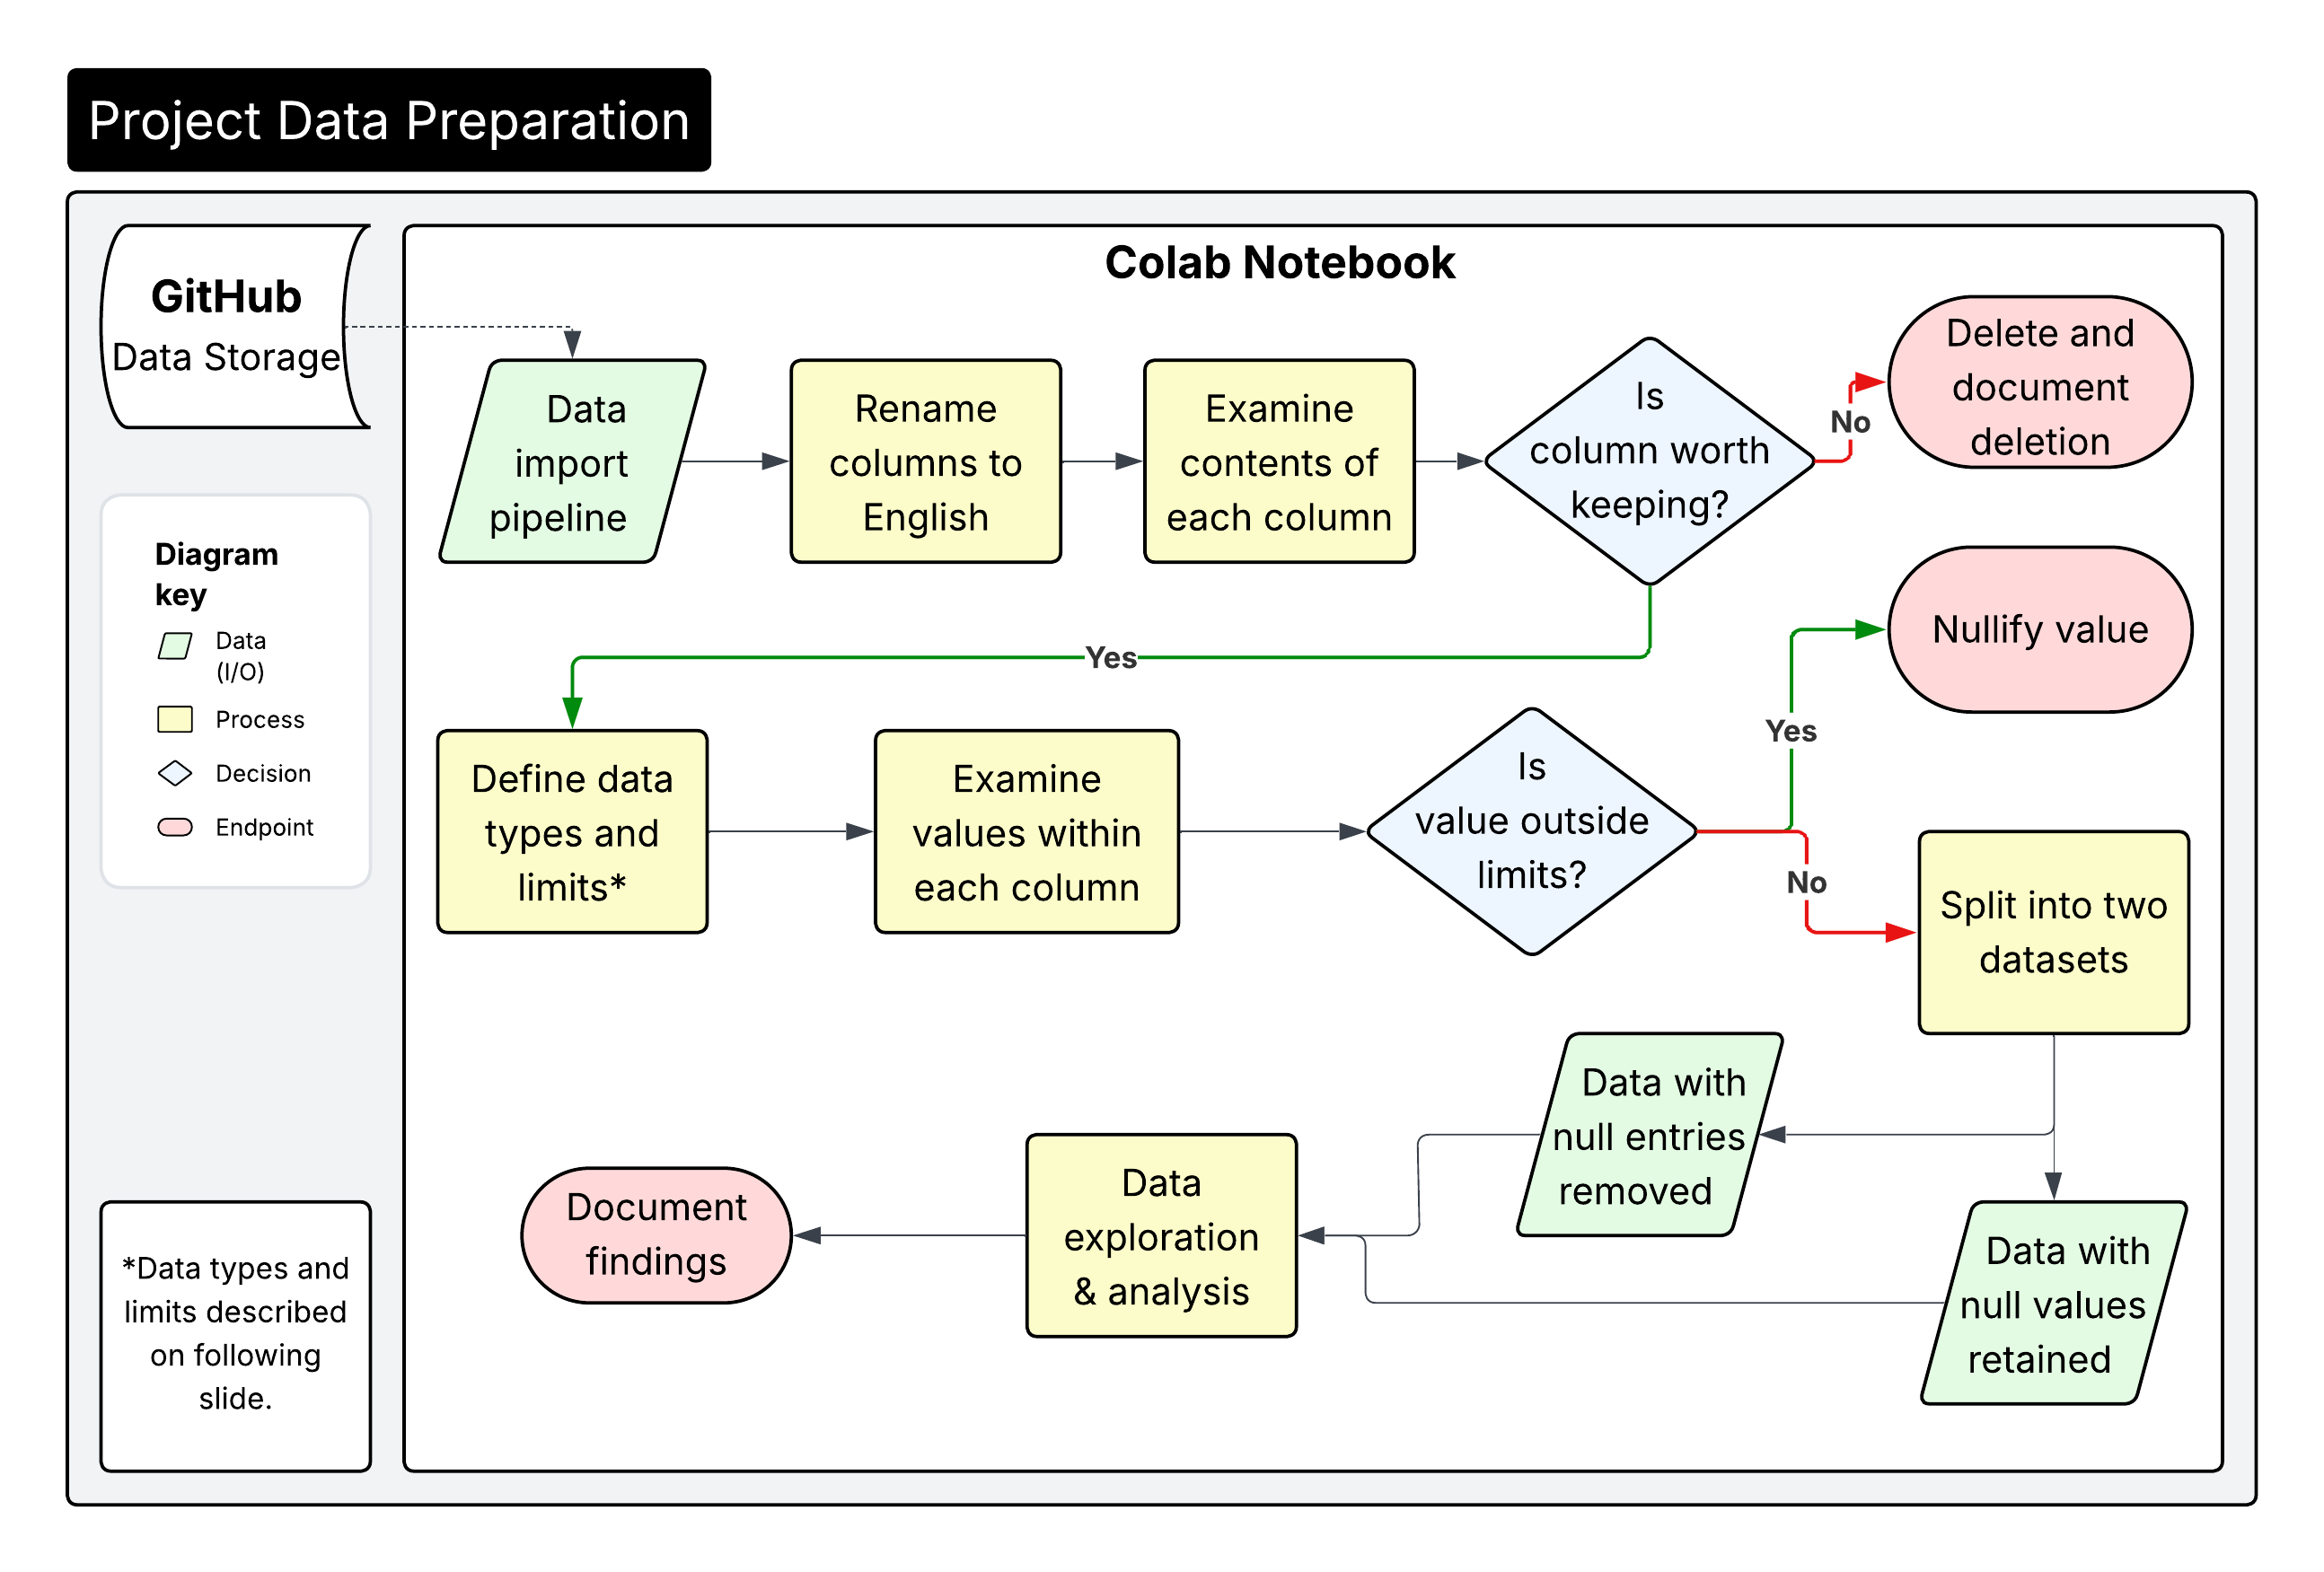
\includegraphics[width=\columnwidth]{data_preparation_pipeline_diagram.png}
\caption{Data preparation pipeline from raw NHIS data through domain validation, feature engineering, and three-tier feature set construction.}
\label{fig:pipeline}
\end{figure}

\begin{figure}[t]
\centering
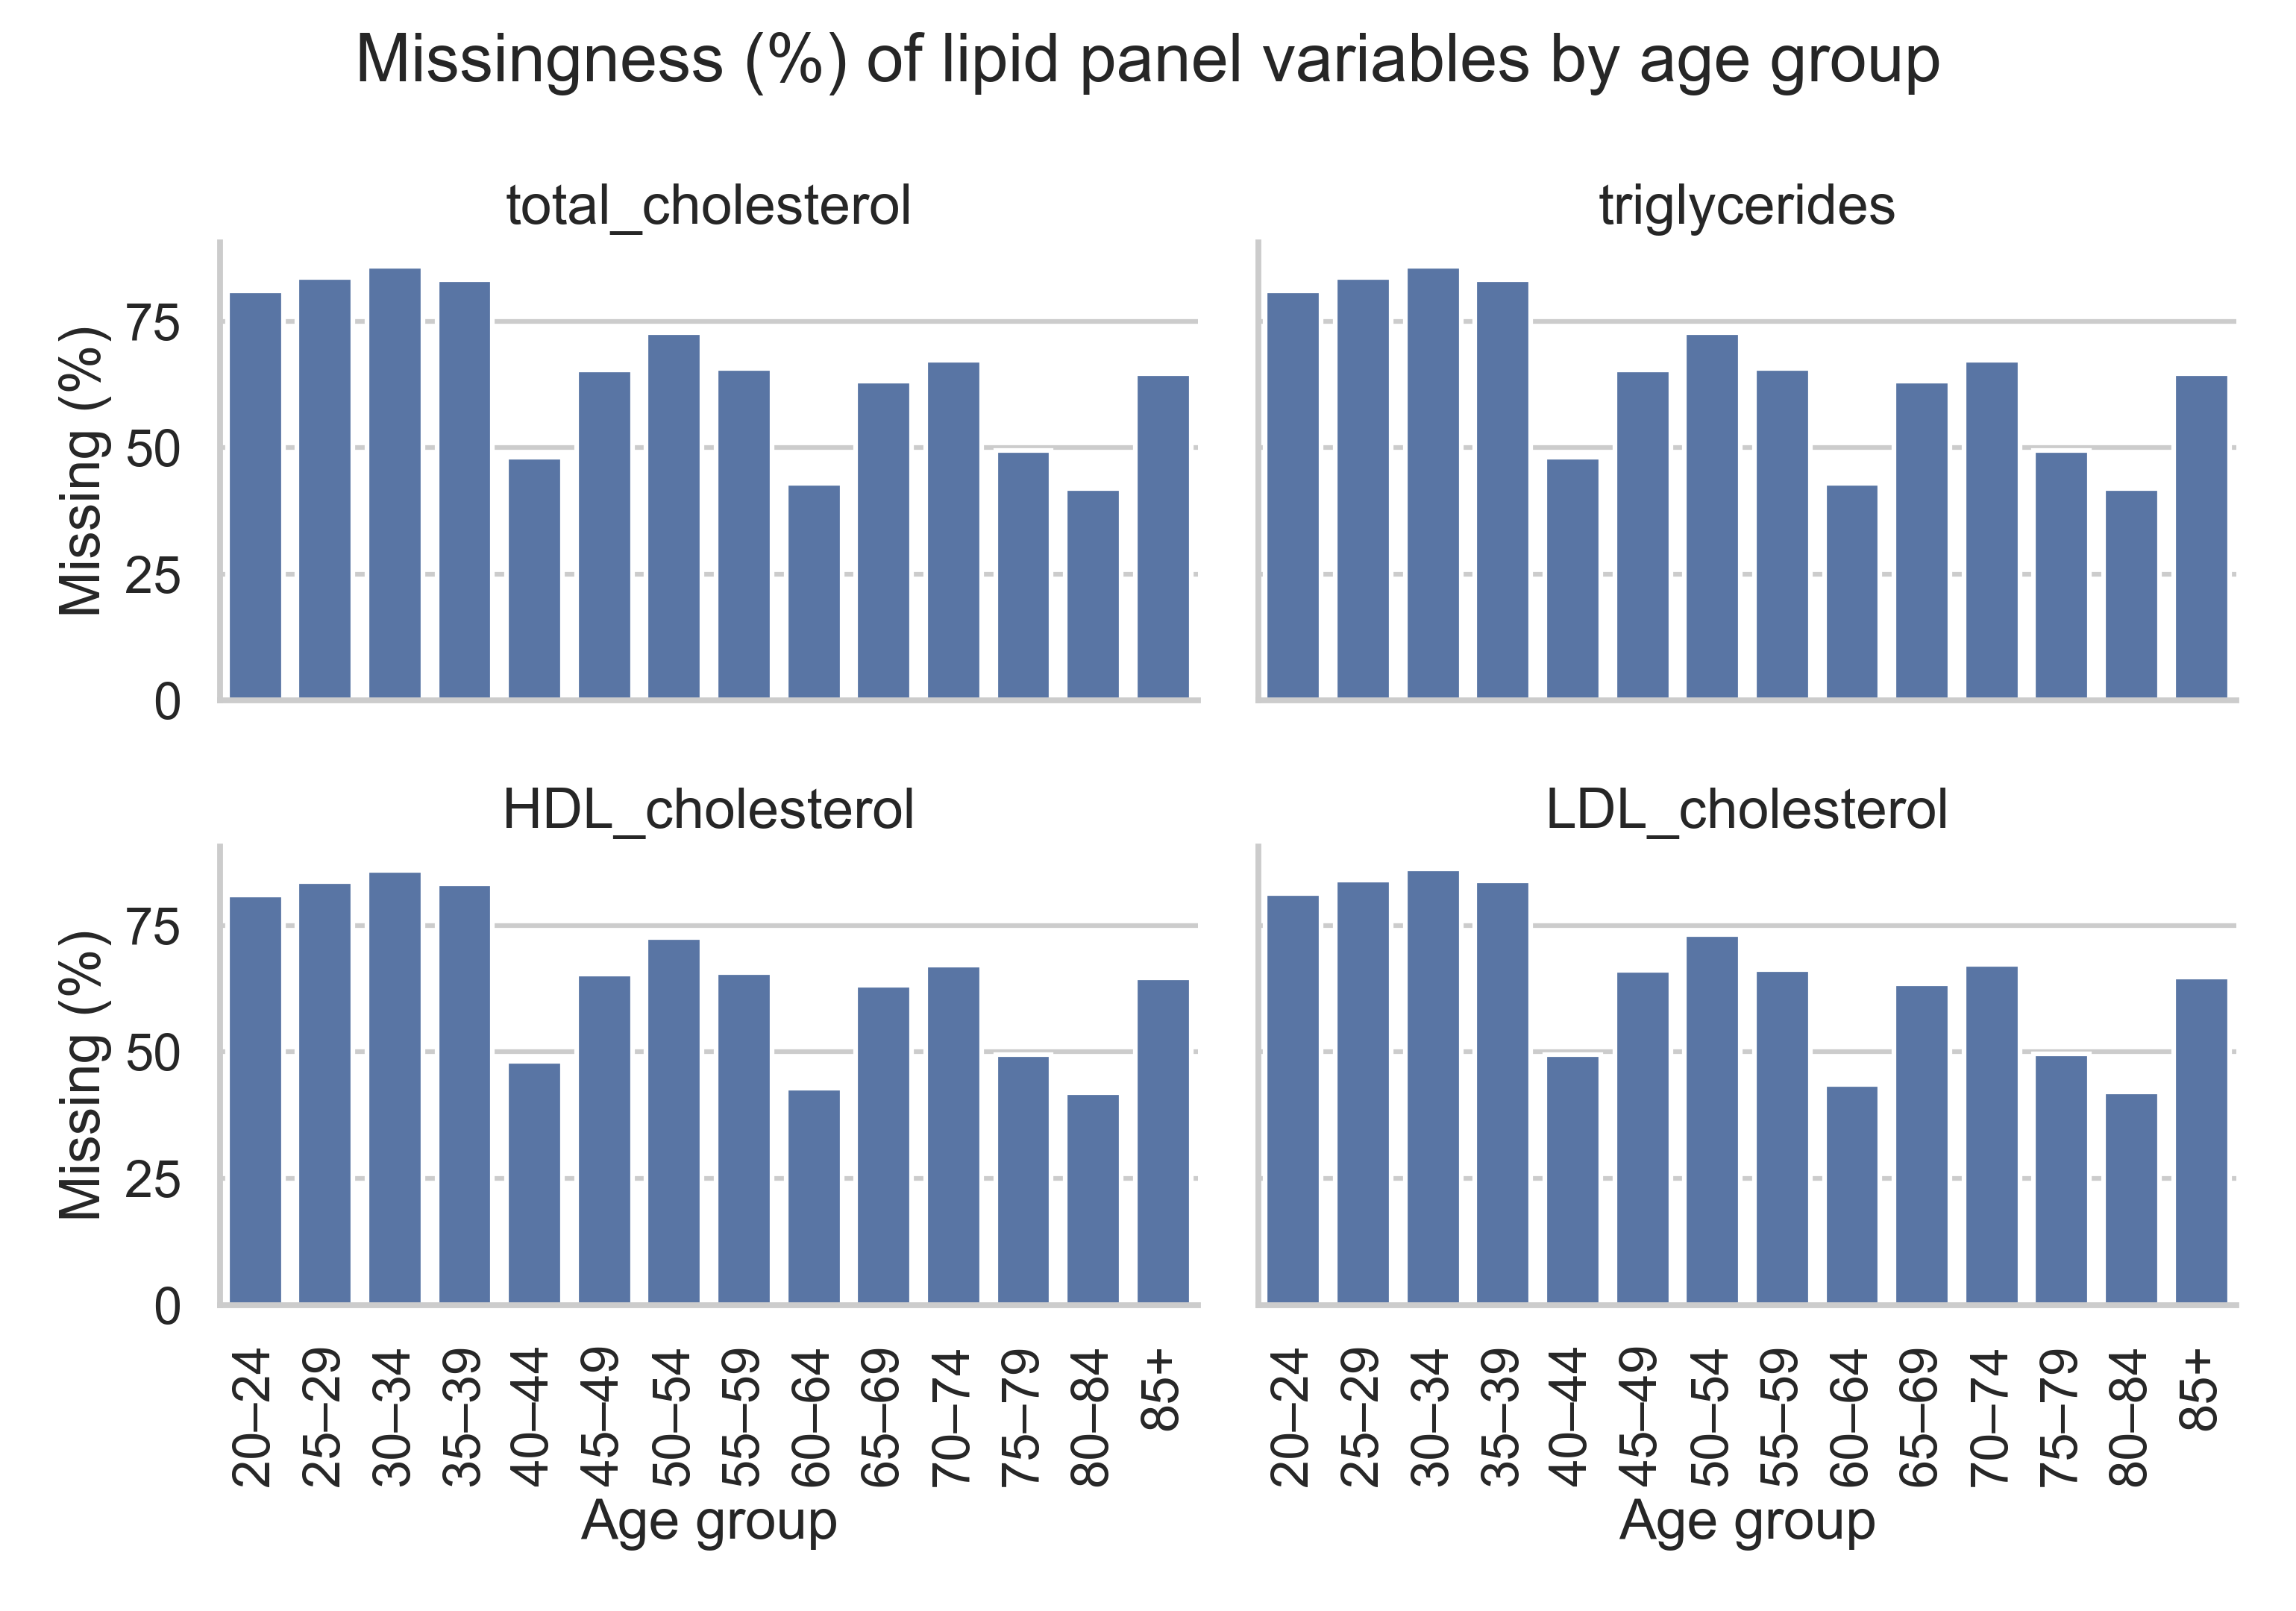
\includegraphics[width=\columnwidth]{lipid_panel_missingness_by_age_facets.png}
\caption{Lipid panel missingness rates by age group. Younger patients are more likely to lack lipid data, reflecting the optional nature of the test.}
\label{fig:missingness}
\end{figure}

\begin{figure}[t]
\centering
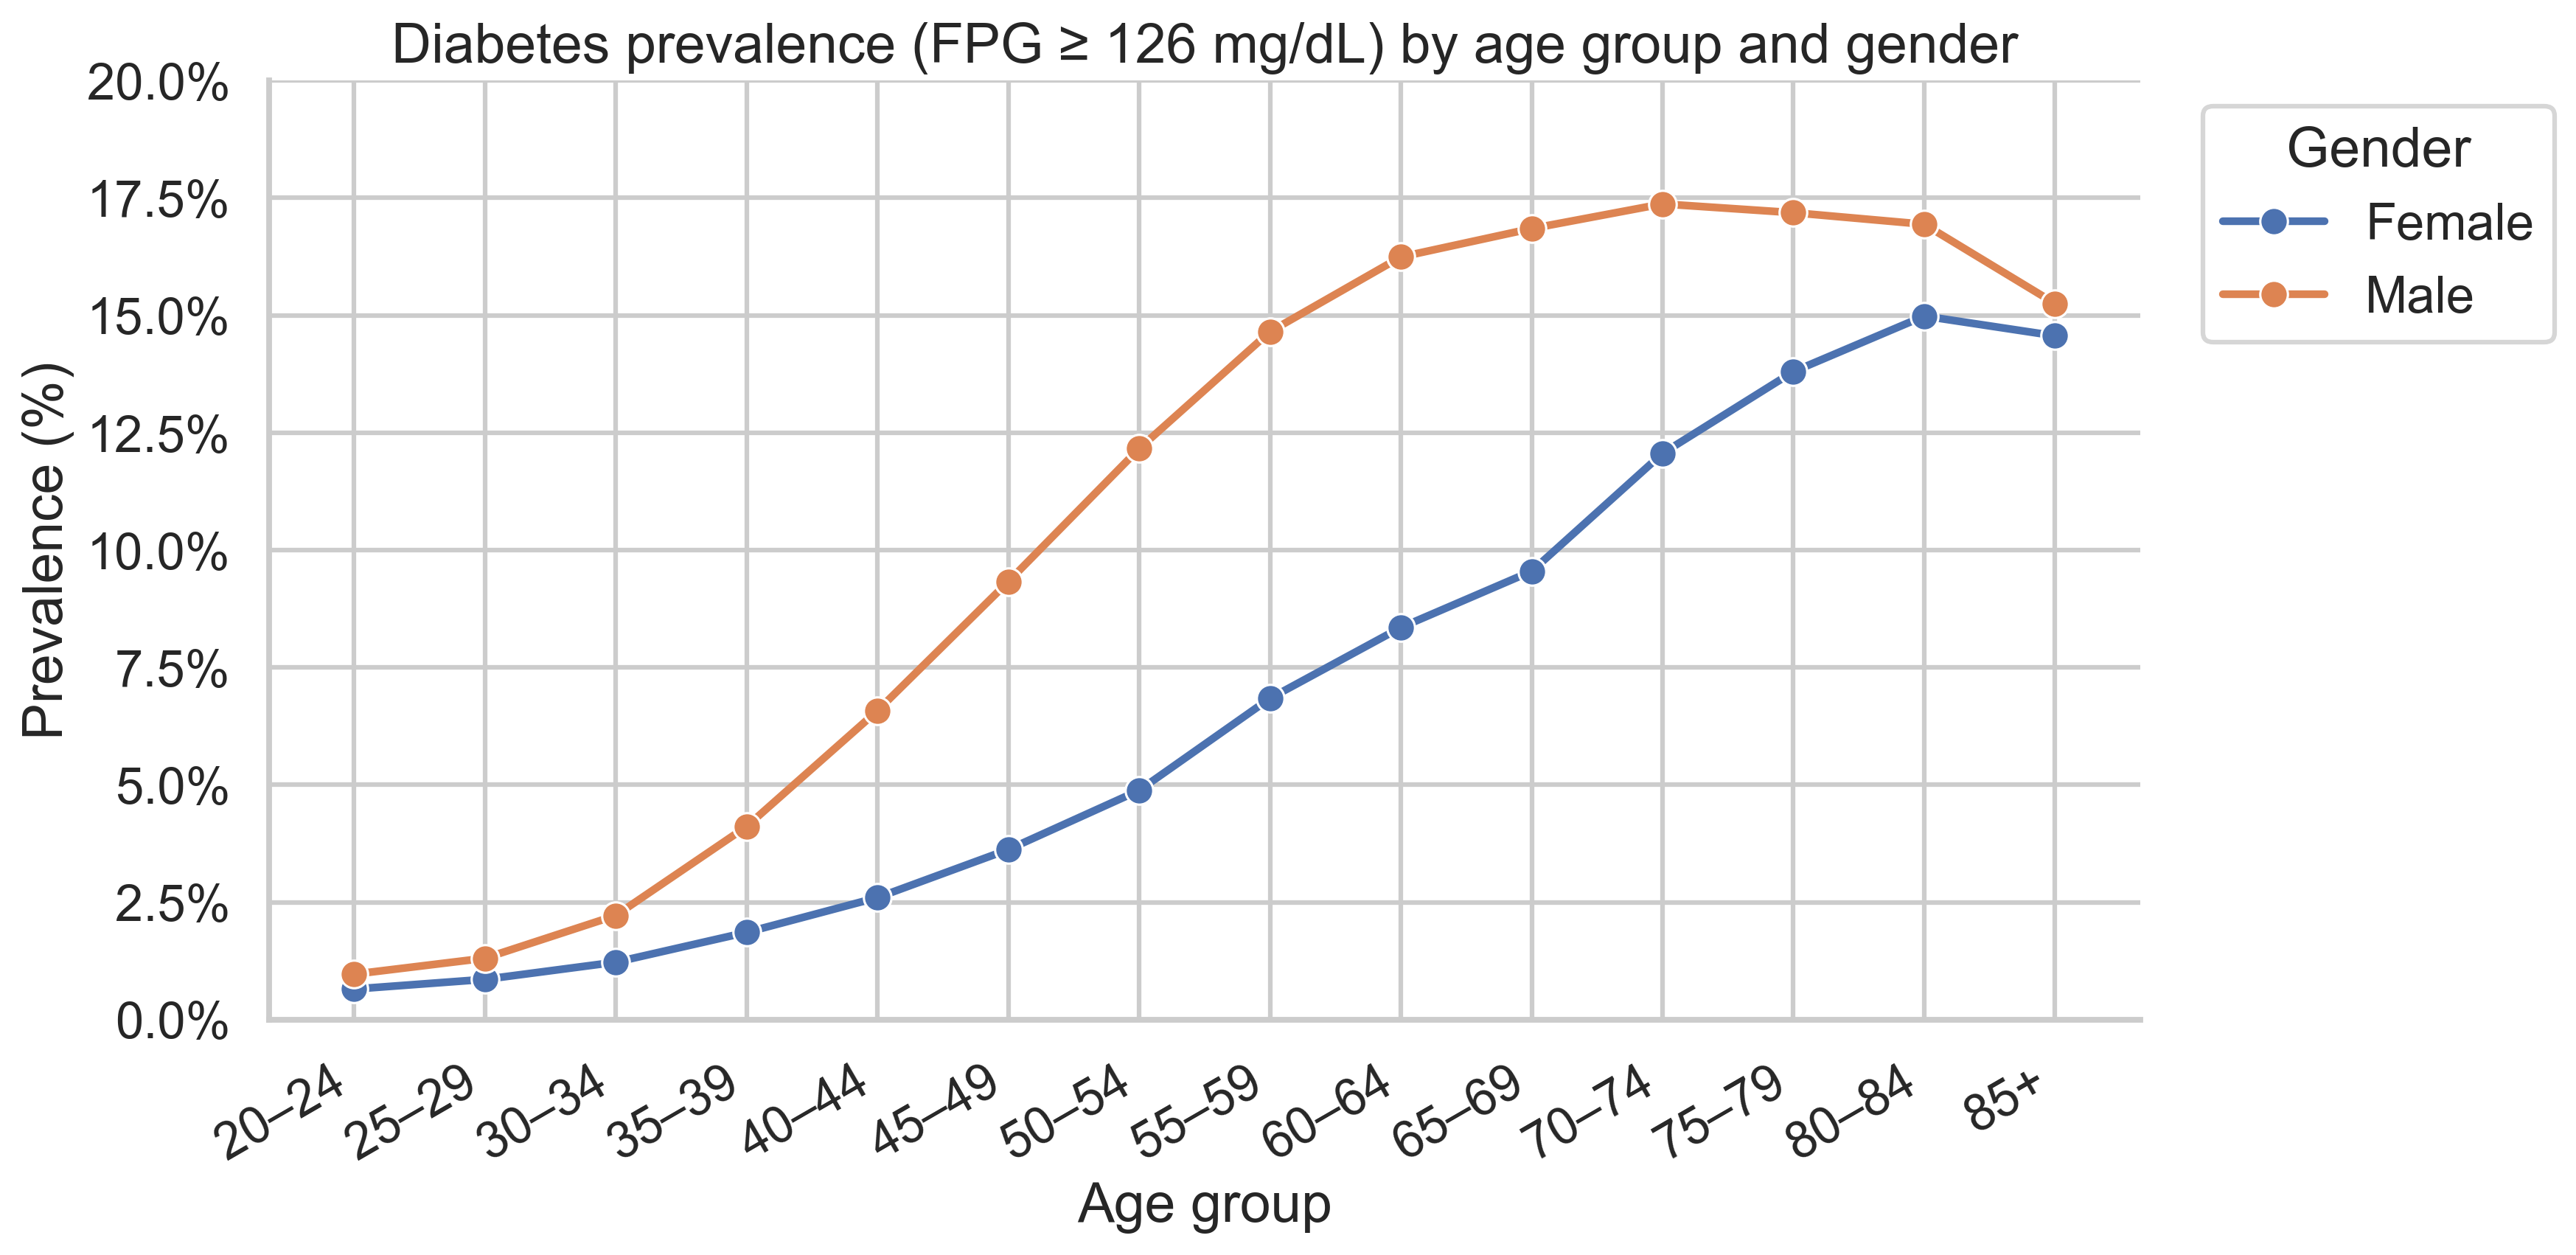
\includegraphics[width=\columnwidth]{diabetes_prevalence_by_age_and_gender.png}
\caption{Distribution of diabetes prevalence by age group and sex in the NHIS 2024 dataset.}
\label{fig:prevalence}
\end{figure}

\section{Methodology}
\label{sec:methodology}

\subsection{Experimental Design}
\label{subsec:experimental-design}

We evaluated eight models on identical stratified splits to ensure a fair comparison. The 994,147 preprocessed records were divided into training (596,487; 60\%), validation (198,830; 20\%), and test (198,830; 20\%) sets using stratified random sampling with a fixed seed of 42, preserving the approximately 7.9\% positive class ratio across all partitions. The split was implemented as an 80/20 outer split followed by a 75/25 inner split of the training portion.

The eight models span three architectural families: gradient-boosted trees (CatBoost in three feature-set configurations), neural networks (a scikit-learn MLPClassifier and a PyTorch Tabular Network with learned categorical embeddings), and linear/tree baselines (Logistic Regression, LinearSVC, and a Decision Tree). All models except the three CatBoost variants operated on the full 40-feature set.

To address the class imbalance (approximately 11.7:1 negative-to-positive ratio), we applied inverse-frequency class weighting $[1.0,\; n_{\text{neg}} / n_{\text{pos}}]$ across most models. The MLPClassifier instead used minority upsampling to a 30\% positive rate during training.

The primary evaluation metric was the Area Under the Receiver Operating Characteristic curve (ROC-AUC), computed on the held-out test set. We selected ROC-AUC because it is threshold-independent and remains informative under class imbalance~\cite{Richardson2024roc}.

\subsection{CatBoost Configuration}
\label{subsec:catboost-config}

CatBoost employs ordered boosting with native categorical feature handling, which mitigates target leakage and eliminates the need for manual one-hot encoding~\cite{Prokhorenkova2018catboost}. These properties make it well suited for clinical screening data containing a mixture of numeric and categorical inputs.

Table~\ref{tab:catboost-hyperparams} summarizes the hyperparameters for the production CatBoost model. The maximum number of boosting iterations was set to 1,500, with early stopping triggered after 100 consecutive rounds without validation-set improvement. The production model selected the checkpoint at iteration 1,324 as its best iteration.

\begin{table}[ht]
\centering
\caption{CatBoost Hyperparameters (Production Model)}
\label{tab:catboost-hyperparams}
\begin{tabular}{ll}
\hline
\textbf{Parameter} & \textbf{Value} \\
\hline
Loss function        & Logloss \\
Max iterations       & 1,500 \\
Learning rate        & 0.03 \\
Tree depth           & 6 \\
L2 regularization    & 5.0 \\
Early stopping       & 100 rounds \\
Best iteration       & 1,324 \\
Random seed          & 42 \\
\hline
\end{tabular}
\end{table}

CatBoost natively handles missing values by learning optimal split directions for absent features during training~\cite{Nijman2022missingdata}. This is particularly important in our dataset, where approximately 66\% of records lack the optional lipid panel. No imputation was performed.

To quantify the marginal contribution of each data category, we trained three CatBoost variants on nested feature subsets: a \emph{Core} model (15 features: 12 numeric demographics and vitals plus 3 categorical indicators), a \emph{Core+Labs} model (26 features: Core plus 6 non-lipid laboratory values and 5 missingness flags), and a \emph{Full} model (40 features: Core+Labs plus 10 lipid-derived features and 4 lipid missingness flags). All three shared identical hyperparameters and training procedures, differing only in the input feature set.

\subsection{Probability Calibration}
\label{subsec:calibration}

Raw CatBoost output probabilities can be poorly calibrated, meaning a predicted probability of 0.10 may not correspond to a true 10\% prevalence in that score band. We applied post-hoc Platt scaling~\cite{Platt1999calibration}, which fits a logistic regression model to the logit-transformed raw probabilities:
\begin{equation}
\label{eq:platt}
P_{\text{cal}}(y=1 \mid x) = \sigma(a \cdot \text{logit}(\hat{p}(x)) + b),
\end{equation}
where $\hat{p}(x)$ is the raw CatBoost output, $\sigma$ is the sigmoid function, and the parameters $a$ and $b$ are fitted on the validation set.

Because Platt scaling is a monotonic transformation, it preserves the ranking of predictions and leaves ROC-AUC unchanged. The calibrated model achieved a Brier score of 0.0643 on the test set, confirming improved reliability of the output probabilities. Calibration quality was assessed visually via a reliability diagram comparing pre- and post-calibration curves against the diagonal.

\subsection{Clinical Threshold Selection}
\label{subsec:threshold}

In a screening context, a false negative (missed diabetes) carries substantially greater clinical cost than a false positive (an unnecessary follow-up blood test). We therefore optimized for high sensitivity rather than balanced accuracy.

The operating threshold was selected as the lowest calibrated probability achieving at least 85\% recall on the validation set, with ties broken in favor of higher precision. This procedure yielded an operating threshold of 0.0659. At this threshold on the held-out test set, the model achieved 85.2\% sensitivity, 62.5\% specificity, 16.3\% positive predictive value (PPV), and 98.0\% negative predictive value (NPV). The low PPV is expected given the 7.9\% base rate and the deliberately recall-oriented threshold; a negative prediction rules out diabetes with high confidence.

\subsection{Interpretability}
\label{subsec:interpretability}

Clinical adoption of machine learning models requires transparency in how predictions are formed~\cite{Deng2025highauc}. We used SHapley Additive exPlanations (SHAP)~\cite{Lundberg2017shap} to attribute each prediction to individual feature contributions.

For the production CatBoost model, we computed exact Shapley values using TreeSHAP, which exploits the tree structure for polynomial-time computation. SHAP values were calculated on a random subsample of 5,000 test-set observations. Global feature importance was derived by averaging the absolute SHAP values across this sample, yielding a ranked list of the features most influential in the model's predictions (reported in Section~\ref{sec:results}).

\subsection{Deployment}
\label{subsec:deployment}

To bridge the gap between a trained model and practical clinical use, we developed an end-to-end screening application. The backend is a FastAPI service that loads the production CatBoost model and Platt calibrator, accepts patient feature vectors via a REST API, and returns both a calibrated probability and a categorical risk tier. The frontend is a lightweight vanilla JavaScript interface designed for use by physicians or community health workers: the user enters available patient data, and the tool returns an interpretable risk assessment.

Rather than presenting a single binary classification, the application assigns each patient to one of four risk tiers derived from the distribution of calibrated probabilities on the held-out test set. Table~\ref{tab:risk-tiers} defines the tier boundaries.

\begin{table}[ht]
\centering
\caption{Risk Tier Definitions}
\label{tab:risk-tiers}
\begin{tabular}{llc}
\hline
\textbf{Tier} & \textbf{Quantile Range} & \textbf{Calibrated Probability} \\
\hline
Low       & 0--50th percentile   & $[0.0,\; 0.0457]$ \\
Moderate  & 50--80th percentile  & $(0.0457,\; 0.1376]$ \\
High      & 80--95th percentile  & $(0.1376,\; 0.2610]$ \\
Very High & 95--100th percentile & $(0.2610,\; 1.0]$ \\
\hline
\end{tabular}
\end{table}

These quantile-based boundaries provide a clinically meaningful stratification. A ``Low'' risk patient falls below the population median probability and may require no immediate follow-up, while a ``Very High'' risk patient is in the top 5\% and warrants prompt confirmatory blood glucose testing. The tiered output also accommodates partial data: because CatBoost handles missing features natively, a health worker can submit whatever fields are available, and the system will still produce a valid risk estimate with an appropriate warning about reduced confidence when key laboratory values are absent.

\section{Results}
\label{sec:results}

We evaluated all eight models on the held-out test set ($n = 198{,}830$) using identical stratified splits (seed = 42). This section reports the model comparison, feature-set ablation, operating characteristics at the screening threshold, SHAP-based feature importance, and post-hoc calibration.

\subsection{Eight-Model Comparison}
\label{sec:results-comparison}

Table~\ref{tab:model-comparison} summarizes ROC-AUC for all eight models. ROC-AUC is appropriate here because it evaluates ranking quality independently of the class imbalance~\cite{Richardson2024roc}.

\begin{table}[ht]
\centering
\caption{Test-set ROC-AUC for all eight models. All models except the CatBoost ablation variants use the full 40-feature set.}
\label{tab:model-comparison}
\begin{tabular}{llc}
\hline
\textbf{Model} & \textbf{Features} & \textbf{ROC-AUC} \\
\hline
CatBoost (Full)          & 40 & \textbf{0.817} \\
PyTorch Tabular Net      & 40 & 0.816 \\
sklearn ANN/MLP          & 40 & 0.812 \\
CatBoost (Core+Labs)     & 26 & 0.808 \\
Logistic Regression      & 40 & 0.792 \\
SVM (LinearSVC)          & 40 & 0.792 \\
Decision Tree            & 40 & 0.776 \\
CatBoost (Core Only)     & 15 & 0.775 \\
\hline
\end{tabular}
\end{table}

The top three models---CatBoost, PyTorch Tabular Net, and the sklearn MLP---achieved ROC-AUC values within 0.005 of each other despite fundamentally different architectures (gradient-boosted trees vs.\ neural networks). The linear models (Logistic Regression and LinearSVC) tied at 0.792, approximately 0.025 below the ensemble and neural approaches, while the single Decision Tree trailed at 0.776. Fig.~\ref{fig:roc-all} overlays the ROC curves for all eight models.

CatBoost was selected as the production model for three reasons: (1) native exact SHAP value computation via ordered boosting, which supports the clinical transparency requirement; (2) native handling of missing values without imputation; and (3) substantially faster training and inference than the neural alternatives.

\subsection{Feature-Set Ablation}
\label{sec:results-ablation}

To quantify the contribution of each data tier, we trained three CatBoost models with identical hyperparameters on progressively larger feature sets. Table~\ref{tab:ablation} reports the results.

\begin{table}[ht]
\centering
\caption{CatBoost feature-set ablation. Delta is relative to the preceding tier.}
\label{tab:ablation}
\begin{tabular}{lcc}
\hline
\textbf{Feature Set} & \textbf{\# Features} & \textbf{ROC-AUC} \\
\hline
Core Only    & 15 & 0.775 \\
Core + Labs  & 26 & 0.808 (+0.033) \\
Full         & 40 & 0.817 (+0.009) \\
\hline
\end{tabular}
\end{table}

Adding six non-lipid laboratory values (hemoglobin, serum creatinine, AST, ALT, GGT, and derived ratios) to the 15 core features produced the largest single gain (+3.3 percentage points of AUC). Adding the lipid panel yielded only a marginal further improvement (+0.9 pp). Fig.~\ref{fig:roc-ablation} compares the three ROC curves.

This result has practical significance: approximately 66\% of NHIS examinees do not receive a lipid panel. On the 130,256 test-set patients lacking lipid data, the full model achieved an AUC of 0.821, confirming that the lipid features add no predictive value when they are absent and that the Core+Labs tier is sufficient for the majority of the screening population.

\subsection{Operating Characteristics}
\label{sec:results-threshold}

The operating threshold was set at the lowest probability achieving $\geq$85\% sensitivity on the validation set, yielding a threshold of 0.0659. Table~\ref{tab:confusion} reports the test-set confusion matrix at this threshold, and Fig.~\ref{fig:confusion} visualizes it.

\begin{table}[ht]
\centering
\caption{Confusion matrix and derived metrics for the CatBoost production model at the screening threshold of 0.0659. Percentages are of the full test set ($n = 198{,}830$).}
\label{tab:confusion}
\begin{tabular}{lcc}
\hline
 & \textbf{Pred.\ Negative} & \textbf{Pred.\ Positive} \\
\hline
\textbf{Actual Negative} & 114,435 (57.6\%) & 68,701 (34.6\%) \\
\textbf{Actual Positive} & 2,318 (1.2\%)    & 13,376 (6.7\%)  \\
\hline
\end{tabular}
\vspace{4pt}

\begin{tabular}{lclc}
\hline
Sensitivity & 85.2\% & Specificity & 62.5\% \\
PPV         & 16.3\% & NPV         & 98.0\% \\
\hline
\end{tabular}
\end{table}

The model correctly identified 85.2\% of diabetic patients (13,376 of 15,694) while maintaining a negative predictive value of 98.0\%. The trade-off is a false positive rate of 37.5\% (68,701 of 183,136 non-diabetic patients flagged). This is an intentional design choice for a screening context: a false positive results in a follow-up fasting glucose test, whereas a false negative leaves diabetes undetected.

\subsection{SHAP Feature Importance}
\label{sec:results-shap}

We computed global SHAP values~\cite{Lundberg2017shap} using CatBoost's native exact algorithm. Table~\ref{tab:shap} lists the ten most important features by mean absolute SHAP value, and Fig.~\ref{fig:shap} provides the full bar chart.

\begin{table}[ht]
\centering
\caption{Top 10 features by mean $|\text{SHAP}|$ value for the CatBoost production model.}
\label{tab:shap}
\begin{tabular}{clc}
\hline
\textbf{Rank} & \textbf{Feature} & \textbf{Mean $|\text{SHAP}|$} \\
\hline
1  & Age                      & 0.936 \\
2  & AST/ALT ratio            & 0.297 \\
3  & GGT (log)                & 0.268 \\
4  & LDL cholesterol          & 0.215 \\
5  & Hemoglobin               & 0.182 \\
6  & Waist-to-height ratio    & 0.153 \\
7  & AST (log)                & 0.130 \\
8  & Waist circumference      & 0.117 \\
9  & TG/HDL ratio             & 0.114 \\
10 & Pulse pressure           & 0.092 \\
\hline
\end{tabular}
\end{table}

Age dominated all other features, with a mean $|\text{SHAP}|$ of 0.936---more than three times the runner-up (AST/ALT ratio at 0.297). This is consistent with established clinical evidence that T2D risk increases substantially with age. The remaining top features span liver enzyme markers, lipid ratios, anthropometric measures, and hemoglobin, all of which are collected during routine health checkups.

Notably, all nine binary missingness indicator flags had effectively zero SHAP importance (maximum $1.7 \times 10^{-7}$). This confirms that CatBoost's native missing-value handling fully subsumes explicit missingness indicators, rendering them redundant~\cite{Sisk2023imputation}.

\subsection{Calibration}
\label{sec:results-calibration}

Raw CatBoost probabilities were recalibrated using Platt scaling~\cite{Platt1999calibration} fitted on the validation set. Because Platt scaling applies a monotonic logistic transform, the ROC-AUC remained unchanged. Fig.~\ref{fig:calibration} compares the pre- and post-calibration reliability diagrams.

The calibrated model achieved a Brier score of 0.0643 and a precision--recall AUC (PR-AUC) of 0.2734. The relatively low PR-AUC reflects the 7.9\% base rate: even a well-ranking model produces modest precision when the positive class is rare. The Brier score confirms that calibrated probabilities are well-aligned with observed outcome frequencies, which is essential for the risk-tier system presented to clinicians.

\begin{figure}[t]
\centering
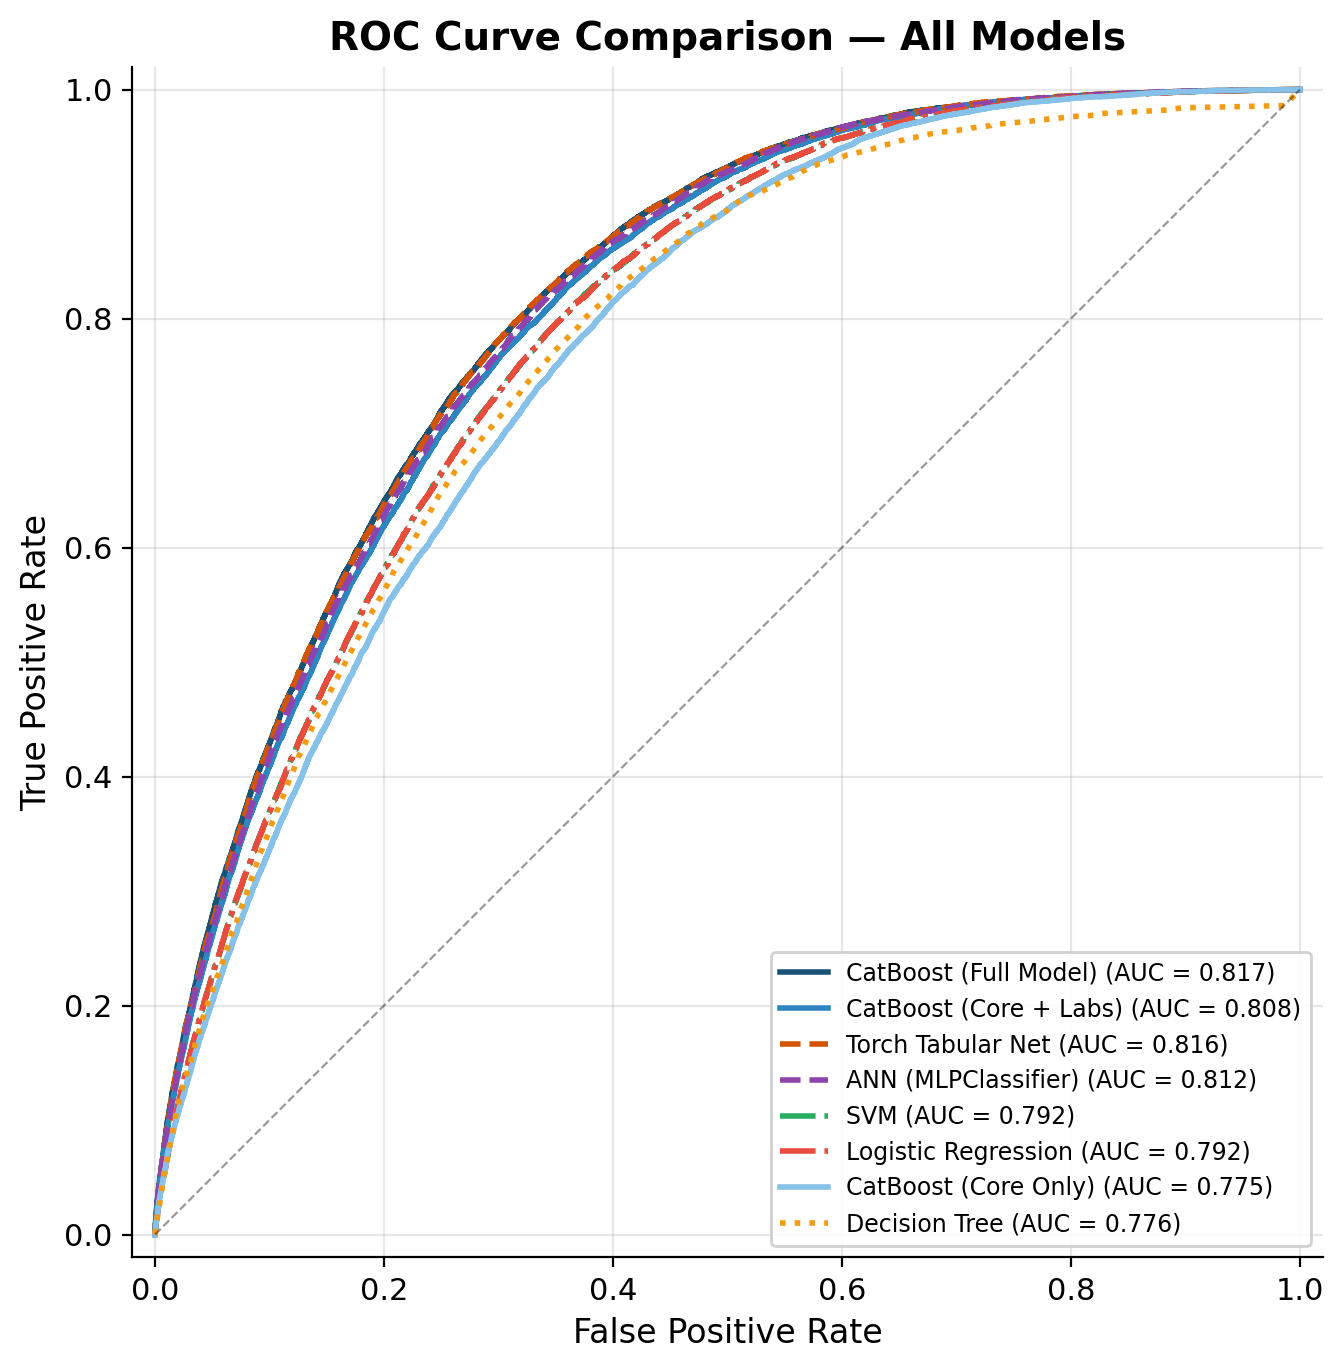
\includegraphics[width=\columnwidth]{roc_all_models.png}
\caption{ROC curves for all eight models on the held-out test set. CatBoost Full (AUC 0.817) is competitive with PyTorch Tabular Net (0.816) and sklearn MLP (0.812).}
\label{fig:roc-all}
\end{figure}

\begin{figure}[t]
\centering
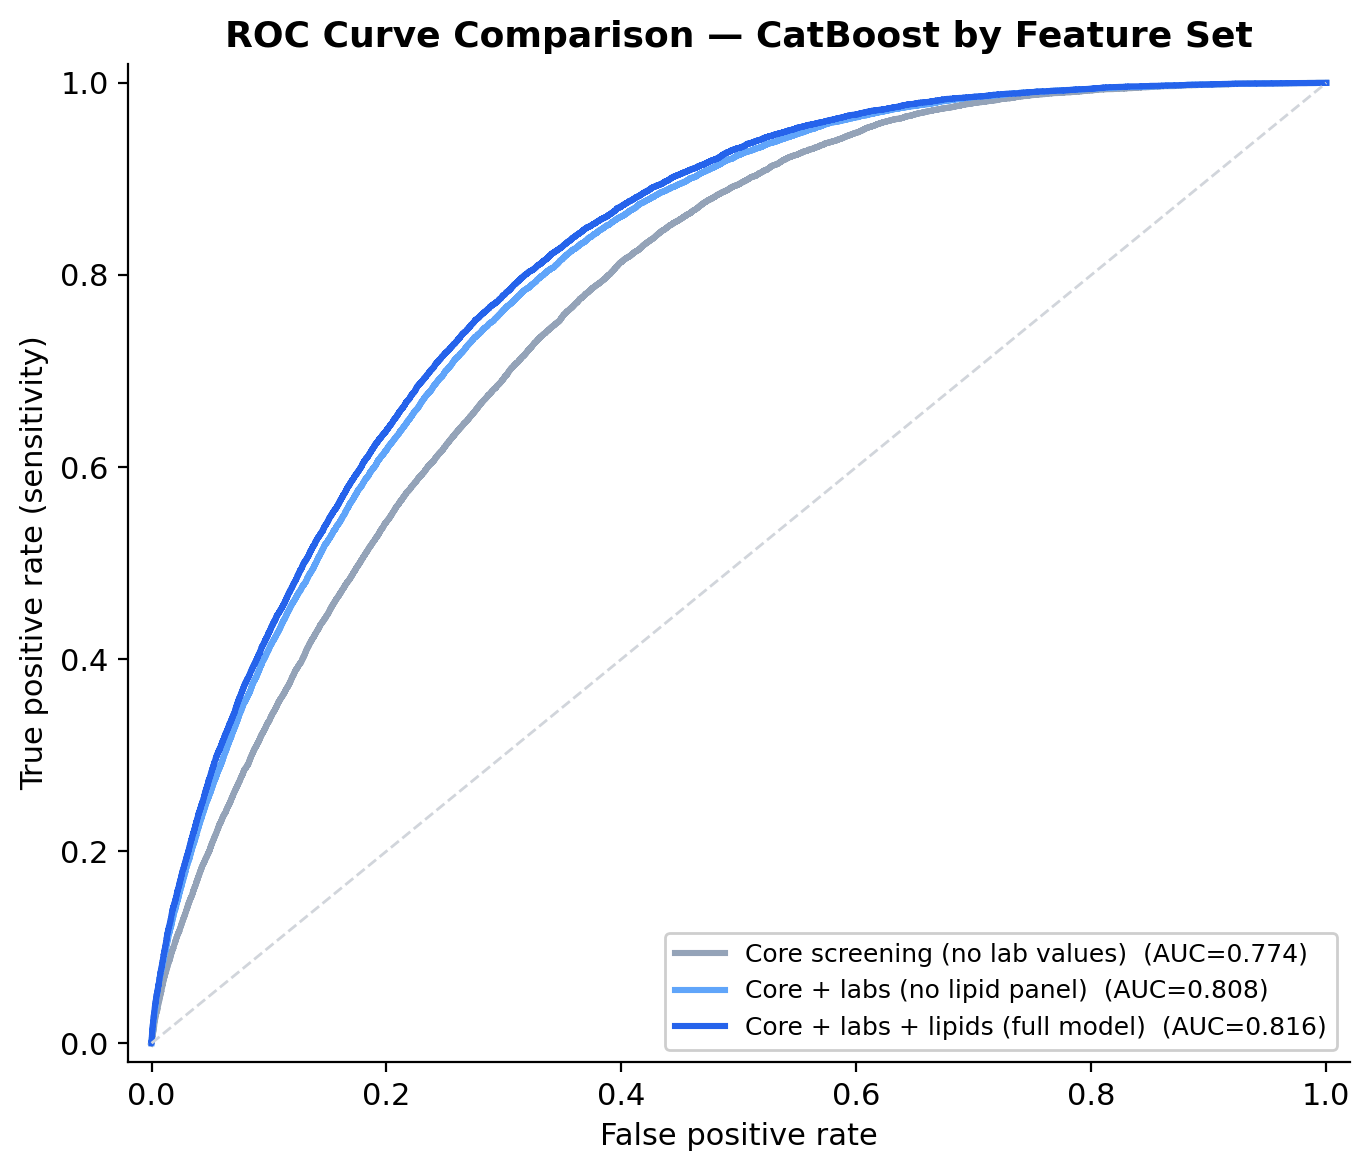
\includegraphics[width=\columnwidth]{catboost_feature_set_roc_comparison.png}
\caption{ROC curves for three CatBoost feature set tiers: Core (0.775), Core+Labs (0.808), and Full (0.817).}
\label{fig:roc-ablation}
\end{figure}

\begin{figure}[t]
\centering
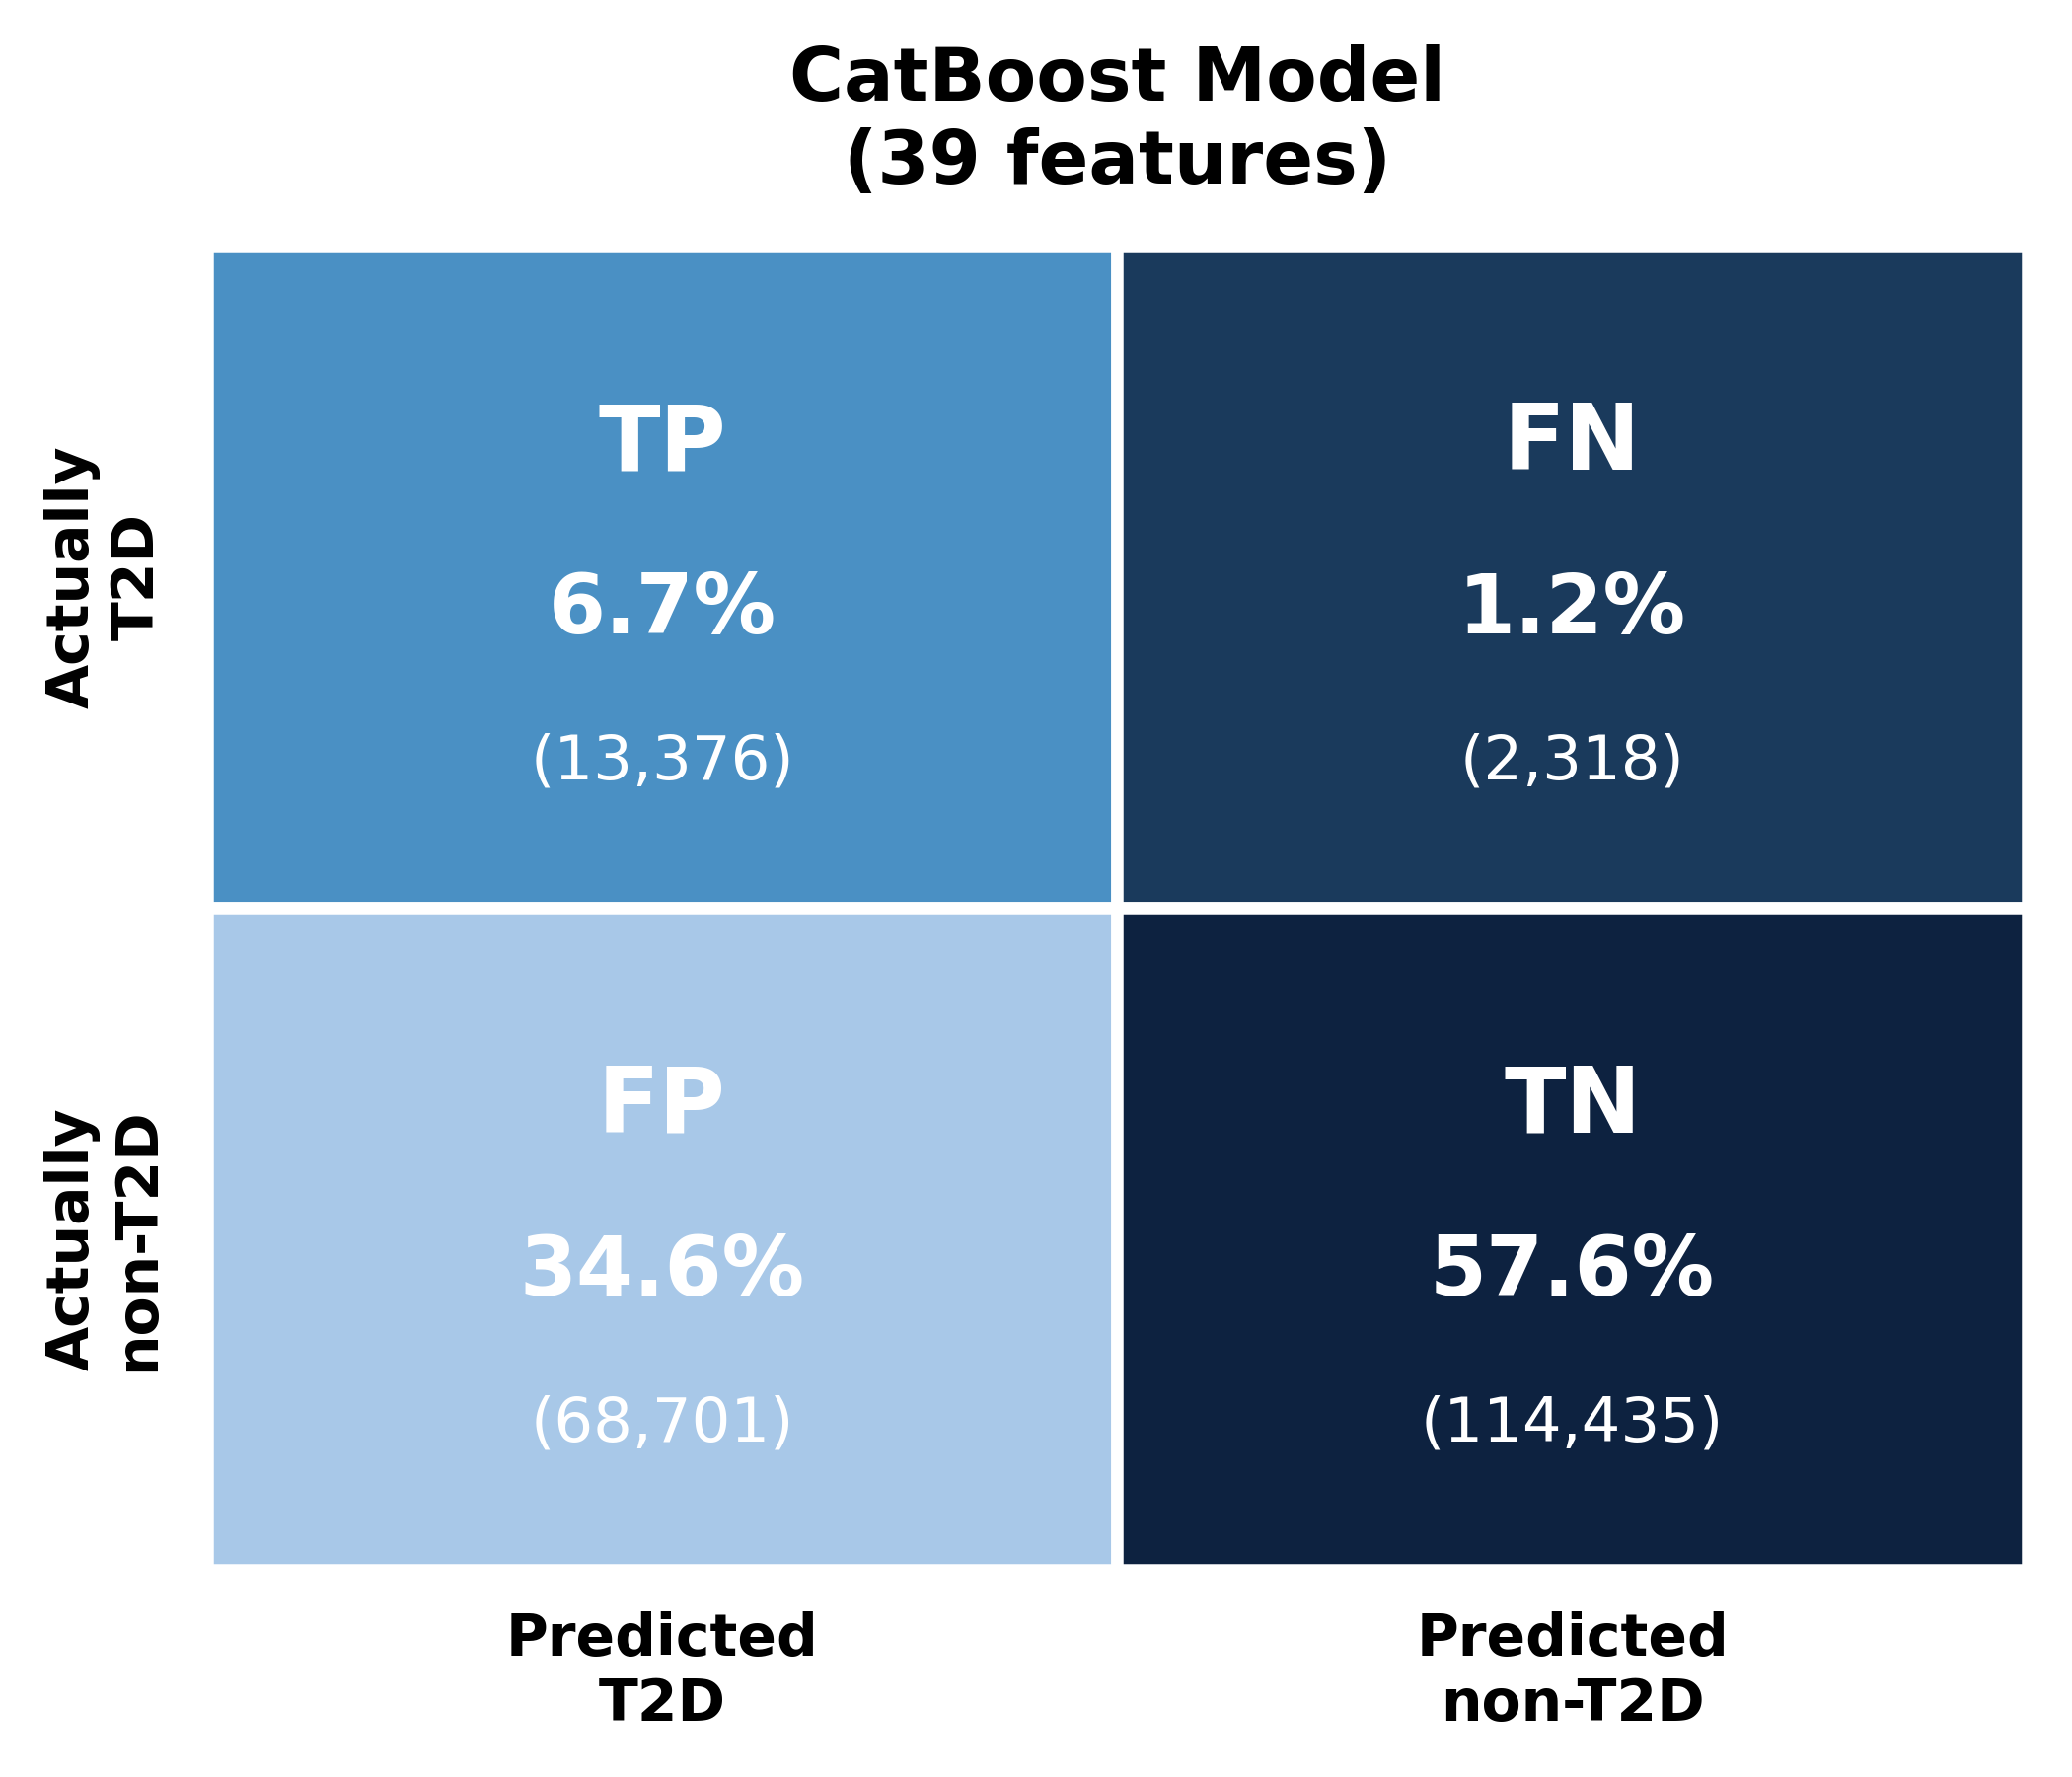
\includegraphics[width=\columnwidth]{catboost_confusion_matrix.png}
\caption{Confusion matrix for the production CatBoost model at the operating threshold of 0.0659. Sensitivity 85.2\%, specificity 62.5\%.}
\label{fig:confusion}
\end{figure}

\begin{figure}[t]
\centering
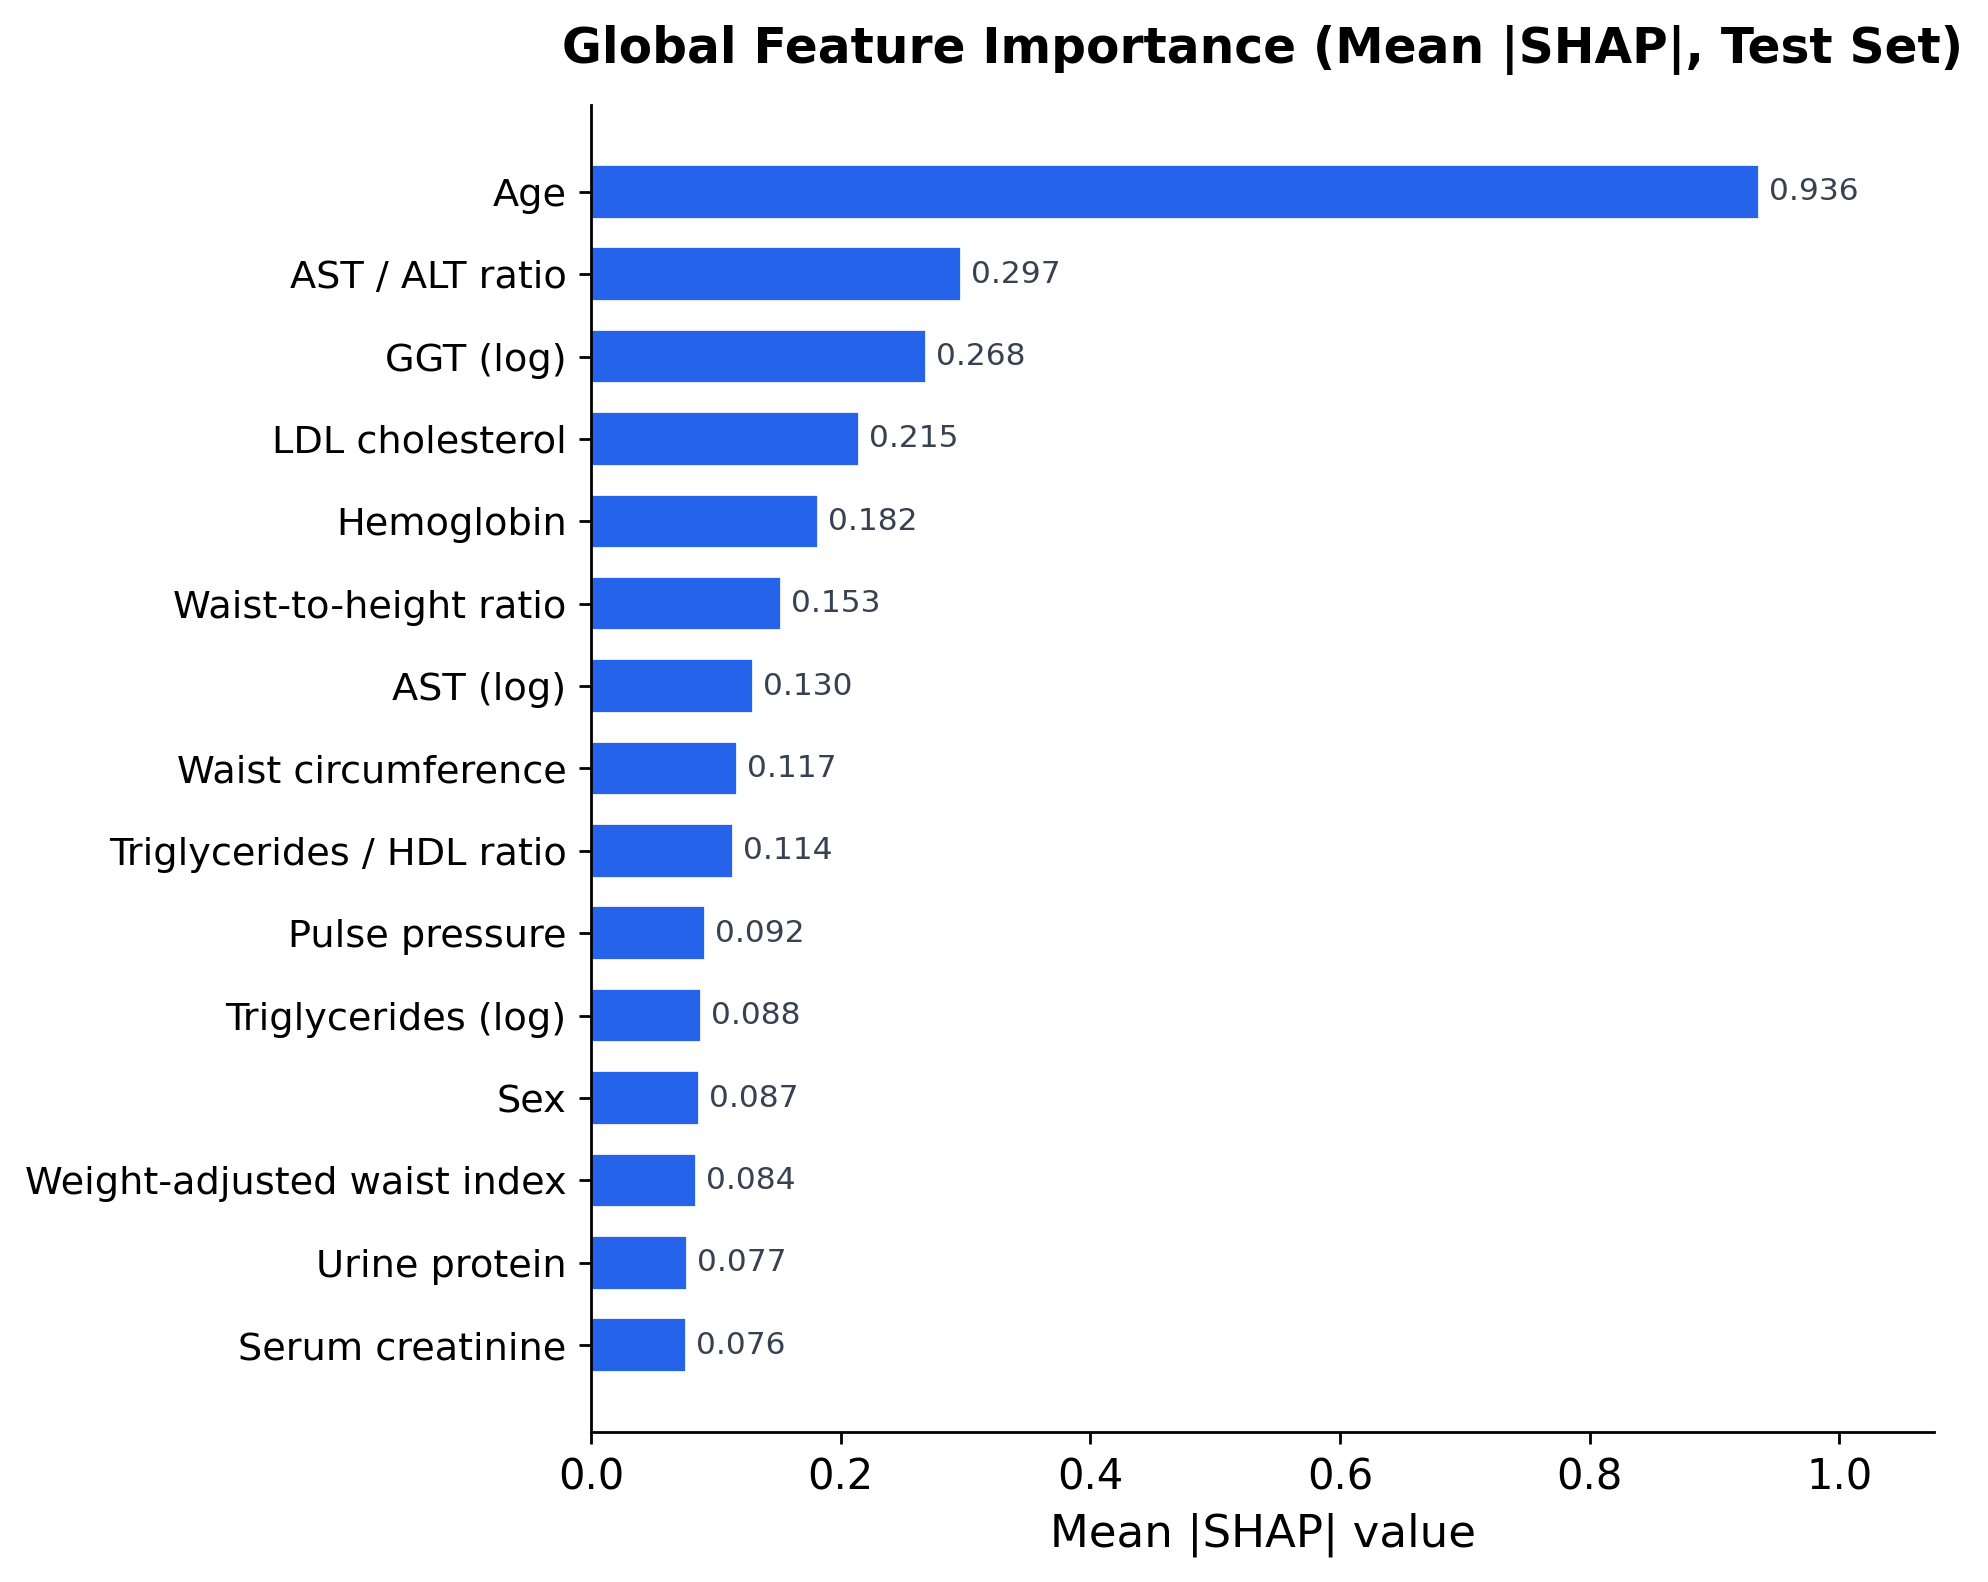
\includegraphics[width=\columnwidth]{shap_importance.png}
\caption{Top 20 features ranked by mean absolute SHAP value. Age dominates (0.936), followed by AST/ALT ratio (0.297) and log GGT (0.268).}
\label{fig:shap}
\end{figure}

\begin{figure}[t]
\centering
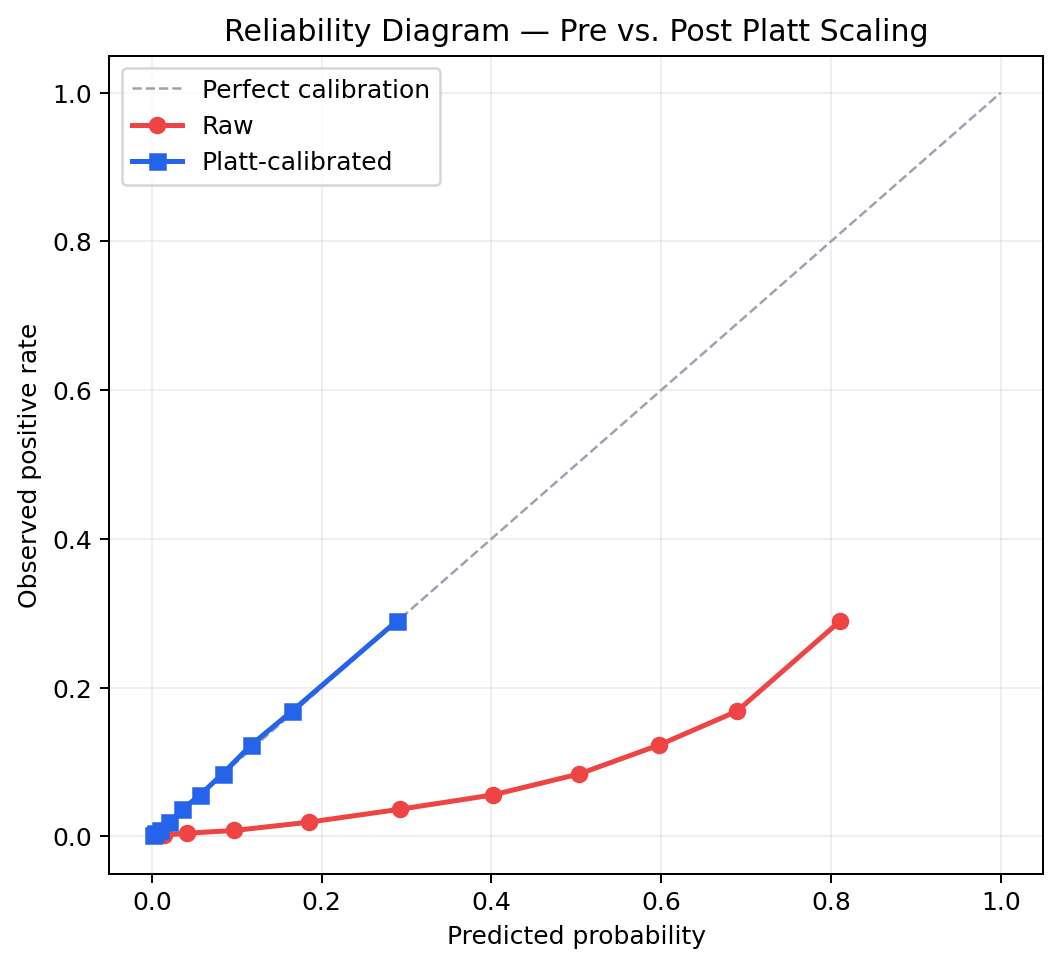
\includegraphics[width=\columnwidth]{calibration_pre_post.png}
\caption{Calibration reliability diagram before and after Platt scaling. Post-calibration probabilities align more closely with observed outcome frequencies.}
\label{fig:calibration}
\end{figure}

\section{Discussion}
\label{sec:discussion}

% Paragraph 1 -- Clinical implications
The operating-point metrics reported in Table~\ref{tab:confusion} have direct implications for population-level screening.
A sensitivity of 85.2\% means that the model identifies the large majority of individuals whose fasting plasma glucose (FPG) exceeds the diabetic threshold, while the 98.0\% negative predictive value (NPV) indicates that patients receiving a negative screen can be reassured with high confidence.
The accompanying false-positive rate of 37.5\% is a deliberate consequence of the recall-oriented threshold: in a screening context, a false positive triggers only a confirmatory blood glucose test, not treatment, making the downstream cost low compared with a missed diagnosis.
Traditional questionnaire-based risk scores such as ADA, IDRS, and FINDRISC have demonstrated lower sensitivity than laboratory-informed models when applied to population screening~\cite{Doddamani2021comparative}, and the USPSTF recommends screening adults aged 35--70 with overweight or obesity~\cite{USPSTF2021screening}, a criterion that misses metabolically unhealthy normal-weight individuals captured by our model's lab-based features.
As Deng et~al.\ emphasize, translating a high area under the receiver operating characteristic curve (AUC) into clinical benefit requires attention to calibration, threshold choice, and deployment context~\cite{Deng2025highauc}; our Platt-calibrated probabilities and recall-targeted threshold address these concerns explicitly.

% Paragraph 2 -- Tree models vs deep learning on tabular data
CatBoost achieved an AUC of 0.817, matching the PyTorch Tabular network (0.816) and the sklearn multilayer perceptron (0.812) within 0.005 AUC (Table~\ref{tab:model-comparison}).
This outcome is consistent with the NeurIPS finding of Grinsztajn et~al.\ that tree-based models match or outperform deep learning on typical tabular datasets~\cite{Grinsztajn2022trees}.
Beyond raw discrimination, CatBoost offers practical advantages for clinical deployment: it provides exact Shapley values through its native TreeSHAP implementation rather than the approximate values produced by model-agnostic methods, it handles missing values internally without requiring a separate imputation step, and it trains and infers substantially faster than neural alternatives.
For a screening tool that must be transparent to clinicians, the alignment of SHAP feature rankings with established risk factors---age, liver enzyme ratios, waist-to-height ratio, lipid ratios (Table~\ref{tab:shap})---is not merely convenient but necessary for building trust and facilitating adoption.

% Paragraph 3 -- Missingness as signal
Approximately 66\% of records in the NHIS dataset lack a lipid panel, reflecting the optional nature of this test in Korean biennial health examinations.
CatBoost handles these missing values natively through learned default split directions, eliminating the need for imputation.
We additionally engineered nine explicit binary missingness flags, yet all exhibited effectively zero SHAP importance (maximum $1.7 \times 10^{-7}$), indicating that the algorithm's internal mechanism fully subsumes the information these indicators were intended to capture.
This finding is consistent with prior work showing that explicit missingness indicators provide limited additional value when the base learner already models absence~\cite{Singh2021missingness, Sisk2023imputation}.
The practical consequence is favorable: the model degrades gracefully in clinical settings that do not routinely order lipid panels, and no external imputation pipeline is required at inference time.

% Paragraph 4 -- Three-tier design and practical deployment
The feature-set ablation in Table~\ref{tab:ablation} reveals an asymmetric cost--benefit structure.
Adding non-lipid laboratory values to the core demographic and anthropometric features produces the largest AUC gain (+0.033, from 0.775 to 0.808), whereas appending the full lipid panel yields only a marginal further improvement (+0.009, to 0.817).
This result carries policy implications: effective T2D screening is achievable without cholesterol tests, reducing per-patient cost and broadening coverage to settings where lipid panels are unavailable.
Even the core-only model (15~features, AUC 0.775) provides useful risk stratification in resource-constrained environments.
The alignment of top SHAP features---age, liver enzymes, waist circumference, lipid ratios---with well-established clinical risk factors supports the model's face validity and suggests that the learned patterns reflect genuine pathophysiological relationships rather than dataset artifacts.
We operationalized these findings in a deployed web-based screening tool that maps calibrated probabilities to a four-tier risk stratification (low, moderate, high, very high), providing clinicians with an actionable output rather than a raw score.
However, the model was trained exclusively on South Korean NHIS data, and its generalizability to other populations---with different dietary patterns, genetic backgrounds, and healthcare delivery structures---remains to be established through external validation.

\section{Limitations and Future Work}
\label{sec:limitations}

Several limitations qualify the interpretation of our results.
First, the model was trained exclusively on South Korean NHIS data; differences in diet, genetic predisposition, and healthcare access across populations mean that discrimination and calibration may not transfer to other countries without retraining~\cite{Sun2022idf}.
Second, the diabetes label is a proxy derived from a single fasting plasma glucose reading (FPG $\geq$ 126~mg/dL) rather than a confirmed clinical diagnosis.
The American Diabetes Association also recognizes HbA1c $\geq$ 6.5\% as a diagnostic criterion~\cite{ADA2024standards}, but HbA1c is not collected in the NHIS general health examination.
This proxy cannot distinguish newly undiagnosed cases from patients with known but poorly controlled T2D, introducing label noise in both directions.
Third, the cross-sectional design identifies individuals who likely have diabetes at the time of the examination; it does not predict future diabetes onset, limiting its use for incident-risk stratification.
Fourth, operating at the recall-oriented threshold produces a 37.5\% false-positive rate (1 $-$ specificity).
Although each false positive triggers only a confirmatory blood test, the downstream cost of additional testing may be substantial when deployed at national scale.
Additionally, all reported metrics derive from a single random seed (42); we did not perform repeated splits or statistical significance testing, so the observed AUC differences between models may fall within sampling variability.
We also did not conduct subgroup analyses stratified by age, sex, or BMI category, which would be necessary to assess whether model performance is equitable across clinically relevant subpopulations.
Finally, patients who lack optional laboratory values may differ systematically from those with complete records---the no-lipid subgroup tends to be younger and healthier---so predictions made with minimal inputs may underestimate risk for atypical patients within that subgroup.

Several directions could address these limitations.
Multi-national validation using cohorts from countries with different demographic and dietary profiles would clarify the model's transferability~\cite{Lee2025multicohort}.
Incorporating longitudinal NHIS records would enable prediction of incident diabetes rather than detection of existing cases.
Integrating the model's calibrated risk score with established screening guidelines such as the USPSTF recommendation~\cite{USPSTF2021screening} or the FINDRISC questionnaire could produce hybrid protocols that leverage both clinical heuristics and data-driven pattern recognition.
On the modeling side, the nine binary missingness indicator flags contributed negligible SHAP importance and could be removed to simplify the feature set without expected performance loss.
Regional calibration of probability thresholds for populations with different baseline prevalence rates would also improve the clinical utility of the risk tiers when the model is applied outside South Korea~\cite{Sun2022idf}.

\section{Conclusion}
\label{sec:conclusion}

This work demonstrates that CatBoost trained on approximately one million Korean NHIS health checkup records with 40 routinely collected features achieves an ROC-AUC of 0.817 for T2D screening, matching neural network architectures while providing native SHAP interpretability. Three-tier feature ablation reveals that strong screening performance persists without lipid panel data (Core+Labs AUC 0.808), with the full lipid panel contributing only a marginal gain of +0.009, an important finding given that lipid tests are optional in many screening programs. At the chosen clinical threshold the model attains 85.2\% sensitivity and 98.0\% negative predictive value, supporting its suitability for population-level triage. SHAP analysis confirms that the most influential predictors---age, liver enzymes, waist circumference, and lipid ratios---align with established clinical risk factors, reinforcing model trustworthiness. The deployed web-based screening tool translates calibrated probabilities into four interpretable risk tiers, requiring no imputation and handling missing data natively. Future work should prioritize multi-national validation to assess generalizability beyond the Korean population and to evaluate performance across diverse healthcare systems.


\section*{Acknowledgments}
This work was conducted as a project for the CDS-492 Capstone in Data Science at George Mason University. The authors thank Dr.\ Mohamed Adel Slamani for his guidance as faculty advisor. We also thank South Korea's National Health Insurance Service (NHIS) for providing healthcare data to the public through the Korean data portal. AI tools including Anthropic's Claude and OpenAI's ChatGPT were used to support development and optimize workflow during the project.

\bibliographystyle{IEEEtran}
\bibliography{references}

\end{document}
